\documentclass{article}

  % packages
    % basic stuff for rendering math
    \usepackage[letterpaper, top=1in, bottom=1in, left=1in, right=1in]{geometry}
    \usepackage[utf8]{inputenc}
    \usepackage[english]{babel}
    \usepackage{amsmath} 
    \usepackage{amssymb}
    \usepackage{amsthm}

    % extra math symbols and utilities
    \usepackage{mathtools}        % for extra stuff like \coloneqq
    \usepackage{mathrsfs}         % for extra stuff like \mathsrc{}
    \usepackage{centernot}        % for the centernot arrow 
    \usepackage{bm}               % for better boldsymbol/mathbf 
    \usepackage{enumitem}         % better control over enumerate, itemize
    \usepackage{hyperref}         % for hypertext linking
    \usepackage{fancyvrb}          % for better verbatim environments
    \usepackage{newverbs}         % for texttt{}
    \usepackage{xcolor}           % for colored text 
    \usepackage{listings}         % to include code
    \usepackage{lstautogobble}    % helper package for code
    \usepackage{parcolumns}       % for side by side columns for two column code
    

    % page layout
    \usepackage{fancyhdr}         % for headers and footers 
    \usepackage{lastpage}         % to include last page number in footer 
    \usepackage{parskip}          % for no indentation and space between paragraphs    
    \usepackage[T1]{fontenc}      % to include \textbackslash
    \usepackage{footnote}
    \usepackage{etoolbox}

    % for custom environments
    \usepackage{tcolorbox}        % for better colored boxes in custom environments
    \tcbuselibrary{breakable}     % to allow tcolorboxes to break across pages

    % figures
    \usepackage{pgfplots}
    \pgfplotsset{compat=1.18}
    \usepackage{float}            % for [H] figure placement
    \usepackage{tikz}
    \usepackage{tikz-cd}
    \usepackage{circuitikz}
    \usetikzlibrary{arrows}
    \usetikzlibrary{positioning}
    \usetikzlibrary{calc}
    \usepackage{graphicx}
    \usepackage{algorithmic}
    \usepackage{caption} 
    \usepackage{subcaption}
    \captionsetup{font=small}

    % for tabular stuff 
    \usepackage{dcolumn}

    \usepackage[nottoc]{tocbibind}
    \pdfsuppresswarningpagegroup=1
    \hfuzz=5.002pt                % ignore overfull hbox badness warnings below this limit

  % New and replaced operators
    \DeclareMathOperator{\Tr}{Tr}
    \DeclareMathOperator{\Sym}{Sym}
    \DeclareMathOperator{\Span}{span}
    \DeclareMathOperator{\std}{std}
    \DeclareMathOperator{\Cov}{Cov}
    \DeclareMathOperator{\Var}{Var}
    \DeclareMathOperator{\Corr}{Corr}
    \DeclareMathOperator{\pos}{pos}
    \DeclareMathOperator*{\argmin}{\arg\!\min}
    \DeclareMathOperator*{\argmax}{\arg\!\max}
    \newcommand{\ket}[1]{\ensuremath{\left|#1\right\rangle}}
    \newcommand{\bra}[1]{\ensuremath{\left\langle#1\right|}}
    \newcommand{\braket}[2]{\langle #1 | #2 \rangle}

  % Custom Environments
    \newtcolorbox[auto counter, number within=section]{theorem}[1][]
    {
      colframe = red!25,
      colback  = red!10,
      coltitle = red!20!black,  
      breakable, 
      title = \textbf{Theorem \thetcbcounter ~(#1)}
    } 
    \newtcolorbox[auto counter, number within=section]{proposition}[1][]
    {
      colframe = red!25,
      colback  = red!10,
      coltitle = red!20!black,  
      breakable, 
      title = \textbf{Proposition \thetcbcounter ~(#1)}
    } 
    \newtcolorbox[auto counter, number within=section]{corollary}[1][]
    {
      colframe = red!25,
      colback  = red!10,
      coltitle = red!20!black,  
      breakable, 
      title = \textbf{Corollary \thetcbcounter ~(#1)}
    } 
    \newtcolorbox[auto counter, number within=section]{definition}[1][]
    {
      colframe = yellow!25,
      colback  = yellow!10,
      coltitle = yellow!20!black,  
      breakable, 
      title = \textbf{Definition \thetcbcounter ~(#1)}
    } 
    \newtcolorbox[auto counter, number within=section]{example}[1][]
    {
      colframe = blue!25,
      colback  = blue!10,
      coltitle = blue!20!black,  
      breakable, 
      title = \textbf{Example \thetcbcounter ~(#1)}
    } 
    \newtcolorbox[auto counter, number within=section]{code}[1][]
    {
      colframe = green!25,
      colback  = green!10,
      coltitle = green!20!black,  
      breakable, 
      title = \textbf{Code \thetcbcounter ~(#1)}
    } 
    \newtcolorbox[auto counter, number within=section]{algo}[1][]
    {
      colframe = green!25,
      colback  = green!10,
      coltitle = green!20!black,  
      breakable, 
      title = \textbf{Algorithm \thetcbcounter ~(#1)}
    } 

    \BeforeBeginEnvironment{example}{\savenotes}
    \AfterEndEnvironment{example}{\spewnotes}
    \BeforeBeginEnvironment{lemma}{\savenotes}
    \AfterEndEnvironment{lemma}{\spewnotes}
    \BeforeBeginEnvironment{definition}{\savenotes}
    \AfterEndEnvironment{definition}{\spewnotes}
    \BeforeBeginEnvironment{corollary}{\savenotes}
    \AfterEndEnvironment{corollary}{\spewnotes}
    \BeforeBeginEnvironment{proposition}{\savenotes}
    \AfterEndEnvironment{proposition}{\spewnotes}
    \BeforeBeginEnvironment{theorem}{\savenotes}
    \AfterEndEnvironment{theorem}{\spewnotes}
    \BeforeBeginEnvironment{exercise}{\savenotes}
    \AfterEndEnvironment{exercise}{\spewnotes}
    \BeforeBeginEnvironment{solution}{\savenotes}
    \AfterEndEnvironment{solution}{\spewnotes}
    \BeforeBeginEnvironment{question}{\savenotes}
    \AfterEndEnvironment{question}{\spewnotes}
    \BeforeBeginEnvironment{code}{\savenotes}
    \AfterEndEnvironment{code}{\spewnotes}
    \BeforeBeginEnvironment{algo}{\savenotes}
    \AfterEndEnvironment{algo}{\spewnotes}

    \definecolor{dkgreen}{rgb}{0,0.6,0}
    \definecolor{gray}{rgb}{0.5,0.5,0.5}
    \definecolor{mauve}{rgb}{0.58,0,0.82}
    \definecolor{darkblue}{rgb}{0,0,139}
    \definecolor{lightgray}{gray}{0.93}
    \renewcommand{\algorithmiccomment}[1]{\hfill$\triangleright$\textcolor{blue}{#1}}

    % default options for listings (for code)
    \lstset{
      autogobble,
      frame=ltbr,
      language=Python,
      aboveskip=3mm,
      belowskip=3mm,
      showstringspaces=false,
      columns=fullflexible,
      keepspaces=true,
      basicstyle={\small\ttfamily},
      numbers=left,
      firstnumber=1,                        % start line number at 1
      numberstyle=\tiny\color{gray},
      keywordstyle=\color{blue},
      commentstyle=\color{dkgreen},
      stringstyle=\color{mauve},
      backgroundcolor=\color{lightgray}, 
      breaklines=true,                      % break lines
      breakatwhitespace=true,
      tabsize=3, 
      xleftmargin=2em, 
      framexleftmargin=1.5em, 
      stepnumber=1
    }

  % Page style
    \pagestyle{fancy}
    \fancyhead[L]{Development Tools}
    \fancyhead[C]{Muchang Bahng}
    \fancyhead[R]{Fall 2024} 
    \fancyfoot[C]{\thepage / \pageref{LastPage}}
    \renewcommand{\footrulewidth}{0.4pt}          % the footer line should be 0.4pt wide
    \renewcommand{\thispagestyle}[1]{}  % needed to include headers in title page

\begin{document}

\title{Development Tools}
\author{Muchang Bahng}
\date{Fall 2024}

\maketitle
\tableofcontents
\pagebreak


This covers computability theory, complexity theory, and automata theory. 
Alphabet. Boolean logic


\section{Text Editing with Neovim} 

  The first thing you do when coding is typing something, and this requires a text editor. Vim is guaranteed to be on every Linux system, so there is no need to install it. However, you may have to install Neovim (which is just a command away). Vim can be a really big pain in the ass to learn, but I got into it when I was watching some video streams from a senior software engineer at Netflix called The Primeagen. He moved around the code like I've never seen, and I was pretty much at the limit of my typing speed, so I decided to give it a try during the 2023 fall semester. My productivity plummetted during the first 2 days (which was quite scary given that I had homework due), but within a few weeks I was faster than before, so if you have the patience, I would recommend learning it. Here is a summary of reasons why I would recommend learning Vim: 
  \begin{enumerate}
    \item It pushes you to know the ins and outs of your editor. As a mechanic with his tools, a programmer should know exactly how to configure their editor.  
    \item The plugin ecosystem is much more diverse than other editors such as VSCode. You can find plugins/extensions for everything. Here is a summmary of them \href{https://github.com/rockerBOO/awesome-neovim\#neovim-lua-development}{here}. 
    \item You're faster. If you're going to be coding for say the next 10 years, then why not spend a month to master something that will make you faster by 10\%? That way, you'll have coded 1 years worth more with a 1 month commitment. I'd take a free 11 months of coding any day. 
    \item Computing clusters and servers will be much easier to navigate since they all run Linux with Vim. 
    \item Vim is lightweight, and you don't have to open up VSCode every time you want to edit a configuration file.  
  \end{enumerate}

  \begin{example}[Vim vs Neovim]
    Experience wise, Vim and Neovim are very similar, and if you configure things rihght, you may not even be able to tell the difference. But there are 3 differences that I want to mention: 
    \begin{enumerate}
      \item Neovim can be configured in Lua, which is much cleaner than Vimscript. 
      \item Neovim provides mouse control right out of the box, which is convenient for me at times and can be easier to transition into, while Vim does not provide any mouse support. 
      \item There are some plugins that are provided in Neovim that are not in Vim. 
    \end{enumerate}
    Either way, the configuration is essentially the same. At startup, the text editor will parse some predetermined configuration file and load those settings. 
  \end{example}

  It may be the case that a remote server does not have neovim installed, or you may not have the permissions to install it. In this case, you can use \textbf{sshfs}, which is a file system client based on the SSH File Transfer Protocol. It allows you to mount a remote directory over SSH. 

\subsection{Configuration Files}

  In Vim, your configuration files are located in \texttt{~/.vimrc} and plugins are located in \texttt{~/.vim/}. In here, you can put in whatever options, keymaps, and plugins you want. All the configuration is written in VimScript. 

  \begin{lstlisting} 
    # options 
    filetype plugin indent on 
    syntax on 
    set background=dark
    set expandtab ts=2 sw=2 ai
    set nu
    set linebreak 
    set relativenumber        
    
    # keymaps
    inoremap <C-j> <esc>dvbi
    inoremap jk <esc>
    nnoremap <C-h> ge
    nnoremap <C-l> w 
  \end{lstlisting}

  In Neovim, I organize it using Lua. It essentially looks for the \texttt{~/.config/nvim/init.lua} file and loads the options from there. We also have the option to import other Lua modules for better file structure with the \texttt{require} keyword. The tree structure of this configuration file should be the following below. The extra \texttt{user} director layer is necessary for isolating configuration files on multiple user environments.  
  
  The init file is the ``main file'' which is parsed first. I generally don't put any explicit options in this file and reserve it only for require statements. It points to the following (group of) files: 
  \begin{enumerate}
    \item \textbf{options.lua}: This is where I store all my options. 
    \item \textbf{keymaps.lua}: All keymaps. 
    \item \textbf{plugins.lua}: First contains a script to automatically install packer if it is not there, and then contains a list of plugins to download. 
    \item \textbf{Plugin Files}: Individual configuration files for each plugin (e.g. if I install a colorscheme plugin, I should choose which specific colorscheme I want from that plugin). 
    \item \textbf{Filetype Configuration Files}: Options/keymaps/plugins to load for a specific filetype. This helps increase convenience and speed since I won't need plugins like VimTex if I am working in JavaScript. 
  \end{enumerate}

  Once you have your basic options and keymaps done, you'll be spending most of your time experimenting with plugins. It is worth to mention some good ones that I use. 
  \begin{enumerate}
    \item \textbf{Packer} as the essential package manager.  
    \item \textbf{Plenary} 
    \item \textbf{Telescope} for quick search and retrieval of files.  
    \item \textbf{Indent-blankline} for folding. 
    \item \textbf{Neoformat} for automatic indent format. 
    \item \textbf{Autopairs} and \textbf{autotag} to automatically close quotation marks and parantheses. 
    \item \textbf{Undotree} to generate and navigate undo history. 
    \item \textbf{Vimtex} for compilation of LaTeX documents. 
    \item \textbf{Onedark} and \textbf{Oceanic Next} for color schemes. 
    \item \textbf{Vim-Startify} for nice looking neovim startup. 
    \item \textbf{Comment} for commenting visual blocks of code. 
  \end{enumerate}

  It is also worthwhile to see how they are actually loaded in the backend. Each plugin is simply a github repo that has been cloned into \texttt{~/.local/share/nvim/site/pack/packer/}, which contains two directories. The packages in \texttt{start/} are loaded up every time Neovim starts, and those in \texttt{opt/} are packages that are loaded up when a command is called in a certain file (known as lazy loading). Therefore, if you have any problems with Neovim, you should probably look into these folders (and possibly delete them and reinstall them using Packer if needed).

\subsection{Troubleshooting}

  A good test to run is \texttt{:checkhealth}, which checks for any errors or warnings in your Neovim configuration. You should aim to have every (non-optional) warning cleared, which usually involves having to install some package, making it executable and/or adding to \texttt{\$PATH}. 

  If you are getting plugin errors, you can also manually delete the plugin directory in `pack/packer` and run `PackerInstall` to re-pull the repos. This may help. 

\subsection{Language Service Providers} 

  If you were to create a text editor from scratch, you would first want to make a buffer and some external program to analyze this buffer (plus some other text files) concurrently. Things like autocompletion, type checking, and syntax checking may all be taken for granted, but it's not, and these are all provided by the \textbf{language service provider}, also known as \textbf{LSP}. LSPs are specific to each language, such as \texttt{pyright} being the mainstream LSP for Python, and \texttt{ts\_ls} for TypeScript. Some of its services have specific names, and overlap a lot. 
  \begin{enumerate}
    \item \textit{Autocompleting} partially typed words with suggestions based on what you typed so far in the current buffer, or from analyzing existing paths of various directories/files. 
    \item \textit{Linting}, which is a general term for finding issues in your code. 
    \item \textit{Type checking} the correct types of variables to find bugs or edge cases in your code. 
    \item \textit{Symbol searching} variables so that you can jump to where they are declared or defined. 
  \end{enumerate}

  The tricky part about LSPs is that they can get quite heavy in computation. For modern laptops this isn't really a problem. For example, on my Macbook Pro M3 I can have a heavy type checker, full autocompletion of every word,  symbol searching of every variable, and linting across \textit{all} files in my current directory (of up to 50 files), all with no noticeable delay. This was quite nice, until I started working on a remote server offering 4 crappy CPUs to work off of, and this just made coding impossible since all of these processes caused a 1 second delay in my writing. Therefore, depending on where you work, LSPs should be lightweight. The balance between functionality and performance is what I think VSCode does very well compared to Neovim. 

\subsection{Snippets}


\section{Documentation with LaTeX} 

  Latex is a great way to take notes, and while it may be tedious to write it at first, it's a skill that you build up just like when you first wrote the alphabet in kindergarten. If you think you'll be slow at latex forever, don't worry. In a few months I was faster at taking notes with latex than by hand or google docs. 

  I still handwrite notes though during class. Some people handwrite because it helps with retention, but I do it because I often need to reorganize the structure and content of my notes multiple times before I have a clear picture of the entire course. My general system is to handwrite notes for about a month's worth of classes, and then spend a few days thinking about them and adding them to my website.  

  Now let's get back to latex. Most users write on Overleaf, which is a platform that makes latex easier by having all the packages you'll ever need on the cloud, along with a user-friendly GUI. Everything is preconfigured, but that means that your work environment can't really be tailored to the way you like it. I've used Overleaf for about 3 years before I started using Vim, and the lack of Vim keybindings on Overleaf just made me write latex on my local desktop. This allows me to have all my files locally, which I can then store in some remote Github repository.  

  I use the Neovim plugin \textbf{VimTex}, which is installed in my \texttt{plugins.lua} with \texttt{use lervag/vimtex}. Then, you want to install TexLive, which is needed to compile tex files and to manage packages. The directions for TexLive installation is available [here](https://tug.org/texlive/quickinstall.html). Once I downloaded the install files, I like to run \texttt{sudo perl ./install-tl --scheme=small}. Be careful with the server location (which can be set with the \texttt{--location} parameter), as I have gotten some errors. I set \texttt{--scheme=small}, which installs about 350 packages compared to the default scheme, which installs about 5000 packages (~7GB). I also did not set \texttt{--no-interaction} since I want to slightly modify the \texttt{--texuserdir} to some other path rather than just my home directory. 

\subsection{TLMGR}

  Once you installed everything, make sure to add the binaries to PATH, which will allow you to access the \textbf{tlmgr} package manager, which pulls from the CTAN (Comprehensive TeX Archive Network) and gives VimTex access to these executables. Unfortunately, the small scheme installation does not also install the \textbf{latexmk} compiler, which is recommended by VimTex. We can simply install this by running 

  \begin{lstlisting}
    sudo tlmgr install latexmk
  \end{lstlisting}

  Now run \texttt{:checkhealth} in Neovim and make sure that everything is OK, and install whatever else is needed. 

  To install other Latex packages (and even document classes), we can use tlmgr. All the binaries and packages are located in \texttt{/usr/loca/texlive/202*/} and since we're modifying this, we should run it with root privileges. The binaries can also be found here. Let's go through some basic commands: 
  \begin{enumerate}
    \item List all available packages: \texttt{tlmgr list}
    \item List installed packages: \texttt{tlmgr list --only-installed} (the packages with the `i` next to them are installed)
    \item Install a package and dependencies: \texttt{sudo tlmgr install amsmath tikz} 
    \item Reinstall a package: \texttt{sudo tlmgr install amsmath --reinstall}
    \item Remove a package: \texttt{sudo tlmgr remove amsmath} 
  More commands can be found \href{http://tug.ctan.org/info/tlmgrbasics/doc/tlmgr.pdf}{here} for future reference.  
  \end{enumerate}

\subsection{PDF Viewers}

  I will already assume you have a PDF viewer installed. Many operating systems come with their own default PDF viewers, such as Preview for MacOS, Adobe/Edge for Windows, or some other for Ubuntu. So what should you look for in a PDF viewer? That depends on your needs, but as of May 2025 here are mine. 

  \begin{enumerate}
    \item \textit{Customization of keyboard shortcuts}. For example, when I want to scroll down 10 pages, I want to be able to use some keymaps to go there rather than scrolling with my mouse wheel. 
    \item Support for dark mode. Text is generally black on a white background, but this can hurt the eyes especially at night when my room is darker. 
    \item Modifying and viewing comments are nice when people are annotating or editing my work. This is especially useful in collaborative research or when doing literature reviews. 
    \item Ability to fill/sign PDF forms. Not as important but is nice for e-signing. 
  \end{enumerate}
  
  On Arch Linux I use \textbf{zathura}, which is lightweight and also comes with vim motions for navigation. On Mac the most similar is \textbf{Skim}, which also has keybindings and supports a dark mode\footnote{Under Skim, Settings, PDF Display, Invert Colors for Dark Mode}. 

\subsection{Compilation and Debugging}

  From the moment you compile a latex file, there are several files that are generated before the final PDF renders. Let's start with the most basic ones. T

  \begin{definition}[\texttt{paper.log}]
    Log file of the compilation. You should first check this when debugging. 
  \end{definition}

  \begin{definition}[\texttt{paper.aux}]
    This is used for reference information. Mainly, if you use \texttt{\\ref\{\}} but the corresponding \texttt{\\label\{\}} is only later in the document, LaTeX has not seen it and won't look ahead. Instead, each time there is a \texttt{\\label\{\}}, a command gets written to the \texttt{.aux} file. Next time you compile your \texttt{.tex}, that \texttt{.aux} is inputted right before the document gets started, and the command you had written to it then registers the value for \texttt{\\ref\{\}}. 
  \end{definition}

  \begin{definition}[\texttt{paper.synctex.gz}]
    This specifies the synchronization between your PDF and source files. In other words, it allows you to click in the PDF to go to the corresponding line in your source code and vice versa. This can be safely deleted. 
  \end{definition}

  \begin{definition}[\texttt{paper.out}]
    This is used by \texttt{hyperref} to store a list of PDF bookmarks. 
  \end{definition}

  Now there may or may not exist, depending on the packages you use. 

  \begin{definition}[\texttt{paper.toc}]
    If you use \texttt{\\tableofcontents}, this will create a \texttt{.toc} file. 
  \end{definition}

  \begin{definition}[\texttt{paper.bbl/blg}]
    The bbl doc is outputted by biber (or bibtex) and contains the prepared data to be used by biblatex (or natbib). Then the blg is the log files of biber/bibtex. 
  \end{definition}

  \begin{definition}[\texttt{paper.fls}]
    
  \end{definition}


\subsection{Macros}

\subsection{Figures and Tikz}

  After this, you can install Inkscape, which is free vector-based graphics editor (like Adobe Illustrator). It is great for drawing diagrams, and you can generate custom keymaps that automatically open Inkscape for drawing diagrams within LaTeX, allowing for an seamless note-taking experience.  



\section{Version Control with Git} 

  Git is a pretty complex version control tool. It allows you to perform different actions. We'll go over them, starting with the most basic to the most complex. In order to learn this, we should know the structure of the git history. 

\subsection{Local Git Repository} 

  When you do \texttt{git init} in a repository, you are essentially saying that you want to keep track of the history of this repository. This can obviously be done with an undo tree, which comes out-of-box in almost all text editors, but it is much more powerful. 

  \begin{definition}[Local Git Tree]
    The history of our repository is essentially a tree, with each node representing some edits composed of 
    \begin{enumerate}
      \item adding a new file 
      \item modifying a file 
      \item deleting a file
    \end{enumerate} 
    Each node is represented by a hash generated from its previous node and the corresponding edits. You can see your history using  
    \begin{lstlisting}
      git log 
    \end{lstlisting} 
    \texttt{HEAD} is a pointer to the node that reflects the state of your current repository (minus your uncommitted edits), which is usually the most recent node. 
  \end{definition} 

  Unlike most undo trees, these nodes are not added automatically. You must add them manually through a 2-step process. 

  \begin{definition}[Stage]
    You want to take a set of edits and \textbf{stage} them. This essentially tells git that these staged files/lines are going to be a part of the next node. 
  \end{definition}

  \begin{definition}[Commit]
    Then you commit your changes, which does the following. 
    \begin{enumerate}
      \item This takes all of your staged changes and packages them in a node $A$. 
      \item It looks at \texttt{HEAD}, uses \texttt{HEAD}'s hash to generate the hash of $A$, and appends $A$ to \texttt{HEAD} by having $A$ point to \texttt{HEAD}.\footnote{So nodes actually point to \textit{previous nodes}.}
      \item It moves \texttt{HEAD} to $A$. 
    \end{enumerate}
  \end{definition} 

  Therefore, when you make your first commit, you are creating a genesis node from which every other edit will be based off of. Your \texttt{HEAD} then points to this commit. This is great start, and let's add more functionality. 

  \begin{definition}[Checkout a Commit]
    You can move \texttt{HEAD} to point to a specific commit by using 
    \begin{lstlisting}
      git checkout <commit-hash>  # point to this commit  
      git checkout HEAD~N         # point to the commit $N$ nodes before HEAD
    \end{lstlisting} 
    This leaves you in a \texttt{detached head state}, which means that your head is not pointing to the end node. This is useful if you want to 
    \begin{enumerate}
      \item \textit{explore the codebase at a commit's snapshot in time}. 
    \end{enumerate}
  \end{definition} 

  Note that so far, we have described git as a linked list plus some extra head pointer. Adding to this linked list is easy since we are simply adding new edits, but deleting can be very tricky. We will first introduce how to delete the most recent $K$ commits, which is the easiest way to delete. 

  \begin{definition}[Reset] 
    Say that your history is 
    \begin{equation}
      (A) \leftarrow (B) \leftarrow (C) \leftarrow (H \mapsto D)
    \end{equation}  
    If we want to throw away commits $C$ and $D$, we can \textbf{reset} to $B$, which deletes $C, D$ and has $H$ point to $B$, giving us 
    \begin{equation}
      (A) \leftarrow (H \mapsto B)
    \end{equation} 
    \begin{enumerate}
      \item A \textbf{soft reset} means that the edits introduced in $C$ and $D$ will still be kept as unstaged changes, and so you may use them as a starting point to make your next commit. 
      \item A \textbf{hard reset} means that the edits are also completely deleted. 
    \end{enumerate}
  \end{definition} 

  Most beginners in git really know these commands when working with their history, but this is really just a glorified stack. The additional operations can be daunting because they have the risk of introducing \textit{conflicts}. 

\subsection{Conflicts} 

  \begin{definition}[Conflicts]
    A \textbf{conflict} arises when two commits contain edits that change some location independently at the same time. They occur most frequently when working with multiple branches, but they can happen even when working on a single branch. Git will tell you when there is conflict between commits $C$ and $C^\prime$ at a certain location. At this point, you will have to manually go to that location and compare the changes introduced in $C$ and $C^\prime$, called \textbf{hunks}. The conflict looks generally like this. 
    \begin{lstlisting}
      ... some code above 
      <<<<< (C)   # hunk 1
      ========
      >>>>> (C')  # hunk 2
      ... some code below
    \end{lstlisting} 

    In order to fix this conflict, you can  
    \begin{enumerate}
      \item select hunk 1 (and ignore hunk 2)
      \item select hunk 2 
      \item select both hunks (i.e. incorporate both edits) 
      \item manually delete the \texttt{>>>}, \texttt{===}, \texttt{<<<} and directly edit the file to make a custom change that overrides both hunks. 
    \end{enumerate} 
  \end{definition} 

  Choosing the option to fix a conflict may sometimes be complicated, since you may not always want to select the hunk reflected in your most recent changes, because doing that might introduce another conflict in a later commit that actually modified the old code into the new code. 

  \begin{definition}[Revert Commit] 
    Say that you have history
    \begin{equation}
      (C_1) \leftarrow (C_2) \leftarrow (C_3) \leftarrow (H \mapsto C_4)
    \end{equation} 
    You can choose to \textbf{revert} and of the 4 commits above. Given any commit $C$, reverting a commit means that you simply add a new commit $C^\prime$ with the changes that are the exact opposite of $C$. If we want to revert commit $C_2$, our history looks like 
    \begin{equation}
      (C_1) \leftarrow (C_2) \leftarrow (C_3) \leftarrow (C_4) \leftarrow (C_2^\prime)
    \end{equation}  
    So really, we are ``deleting'' our history by adding. 
  \end{definition} 

  \begin{example}[Conflicts in Reverting]
    Say that you have history
    \begin{equation}
      (C_1) \leftarrow (C_2) \leftarrow (C_3) \leftarrow (H \mapsto C_4)
    \end{equation} 
    If you try to revert $H$, this is fine and will never have conflicts. Say that you made an edit in $(C_3)$ where you added $x = 4$ to some python script, and then you removed this line in $(C_4)$. Then if you add $(C_3^\prime)$ to undo it, it tries to delete a line that isn't even there! Therefore you will get a conflict that looks something like 
    \begin{lstlisting}
      <<<<< (C4)   # hunk 1 
      - x = 4 
      ========
      - x = 4
      >>>>> (C3')  # hunk 2
    \end{lstlisting}
    Obviously you can just select either one of the hunks to get what you want. 
  \end{example} 

  Conflicts are unavoidable and you will have to get comfortable with them.  

  \begin{definition}[Amending a Commit]
    If you have some staged edits and you decide that these edits should go into some previous commit rather than a new one, you can \textbf{amend} the old commits. In lazygit, you can stage which edits you want to amend with, then go to the commit in your working branch and press \texttt{<shift-a>} to amend it. 
  \end{definition}

\subsection{Interactive Rebasing} 

  Even though we can revert commits, we haven't actually found out how to truly \textit{delete} a commit from your history which modifies 
  \begin{equation}
    (A) \leftarrow (B) \leftarrow (C) \leftarrow (D)
  \end{equation} 
  to something like 
  \begin{equation}
    (A) \leftarrow (B) \leftarrow (D)
  \end{equation} 

  \begin{definition}[Rebasing]
    Essentially, we want to \textit{directly} (unlike a revert) modify our history that goes \textit{beyond} (unlike a reset) the last $K$ commits. Any actions that modifies the history is known as \textbf{rebasing}, which can be done automatically by git (regular rebasing just picks all commits) but must often be done \textbf{interactively}, which allows for more operations listed below. When you want to start an interactive rebase, you want to tell git from which commit $C_s$ you want to start the interactive rebase on. 
    \begin{lstlisting}
      git rebase -i <start commit hash>
    \end{lstlisting}
    You are saying that from commit $C_s$ and beyond until the end $C_n$, I may arbitrarily modify them, but commits previous to $C_s$ will be untouched. When you do this, all commits $C_i$ where $i \geq s$ will be shown as below. 

    \begin{figure}[H]
      \centering 
      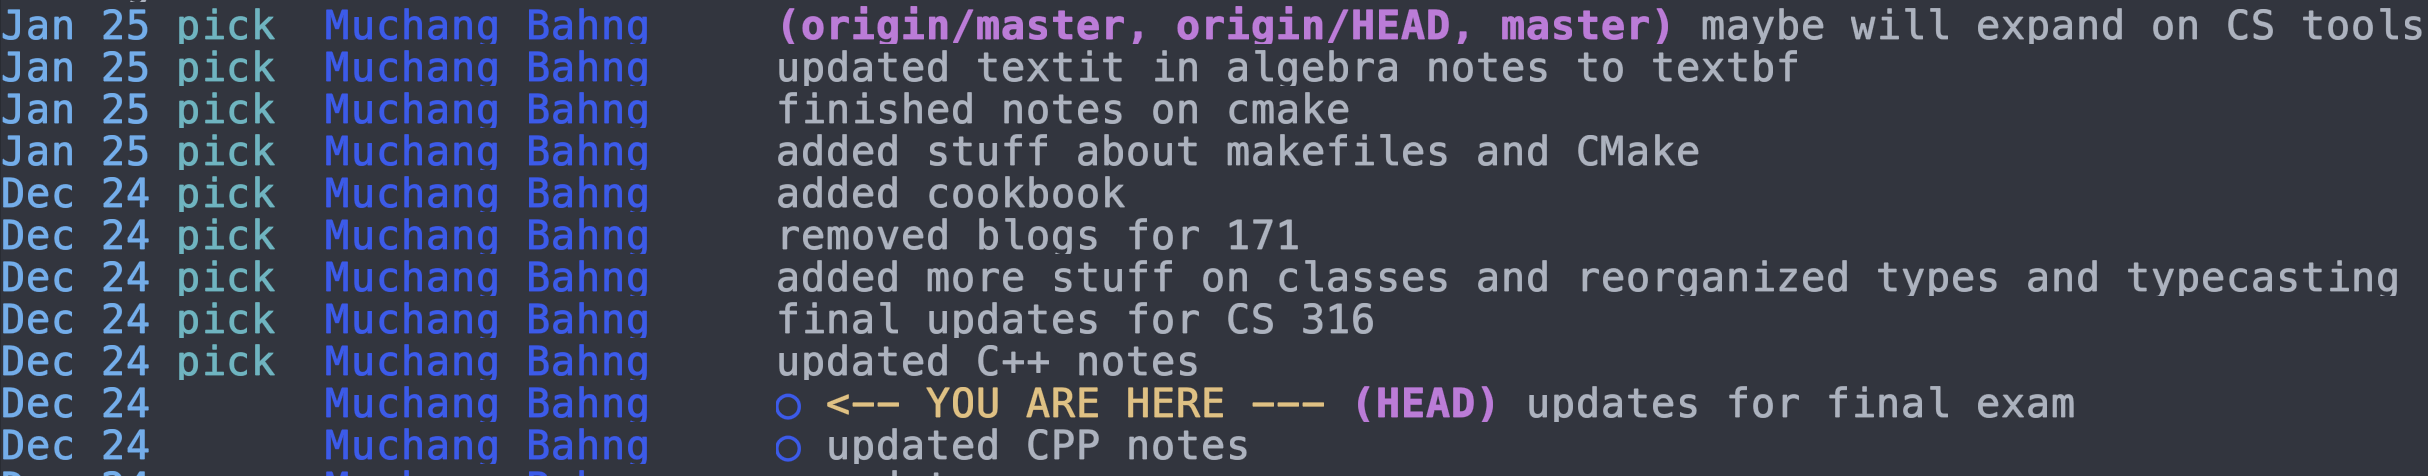
\includegraphics[scale=0.3]{img/rebase.png}
      \caption{Interactive rebase shown in LazyGit.} 
      \label{fig:rebase}
    \end{figure}

    There are a fixed set of supported operations allows in an interactive rebase.\footnote{Note that pick and reword will never cause conflicts. Squash and fixup will most likely not cause conflicts. Drop, break, edit, and swapping may cause conflicts.}
    \begin{enumerate}
      \item \textbf{Pick}. This just means that you are leaving the commit alone, i.e. picking it to be in the rebase. 
      \item \textbf{Reword}. Just edits the commit message. 
      \item \textbf{Squash}. Given commit $C_i \leftarrow C_{i+1}$, you can label $C_{i+1}$ with \texttt{squash} to merge it into $C_{i}$, turning 2 nodes into one. This almost never causes conflicts. The new commit message is just those of $C_{i}, C_{i+1}$ concatenated. 
      \item \textbf{Fixup}. Like squash, but discard the commit's message.  
      \item \textbf{Drop}. This deletes a commit and removes it entirely.  
      \item \textbf{Break}. Stop at this commit to edit it. I think you can change which edits you have committed, choose which edits to keep, and choose which edits to remove (back into your unstaged changes). 
      \item \textbf{Edit}. Stop at this commit to amend it. 
      \item You can also swap commits by editing the text file so that the commits are in a different order. 
        \begin{lstlisting}
          # Original order in rebase editor:
          pick abc123 First commit
          pick def456 Second commit

          # After swapping lines in editor:
          pick def456 Second commit
          pick abc123 First commit 
        \end{lstlisting}
    \end{enumerate} 
    After you edit the rebase text file and continue the rebase, git will do the following sequentially: 
    \begin{enumerate}
      \item \texttt{HEAD}, which pointed at $C_n$, will point towards $C_s$. 

      \item While \texttt{HEAD} is pointing at $C_i \neq C_n$ (i.e. not at the end), we do the following. 
        \begin{enumerate}
          \item It will attempt to perform all the operations you have specified for the next commit $C_{i+1}$. 
          \item If the operations are finished, we increment \texttt{HEAD} to point to $C_{i+1}$ and continue. 
          \item If there is a conflict, it will pause, state that there are conflicts between $\texttt{HEAD} = C_i$ and $C_{i+1}$, and ask you to resolve them. Once resolved it will continue. 
        \end{enumerate} 

      \item Then we are done with the rebase since we have went through all commits, modified them, and resolved all conflicts. 
    \end{enumerate}
    Interactive rebasing is an extremely powerful way to modify your commit history, and it's probably the operation where you'll spend the most time on git. 
  \end{definition} 

  Again, note that if you have changed anything in commit $C_i$, then the hash of $C_i$ every $C_j$ after will get changed. This causes git to interpret these changed commits as completely new ones, even if we only picked a given commit without any modifications. For single-branch rebases, this is fine, but this causes some nasty problems when rebasing over multiple branches, as we will talk about later. 

  \begin{definition}[Patching]
    An easier way to modify your edits in old commits is through \textbf{patching}.\footnote{Though patching really just does an interactive rebase in the backend.} Within a commit, a \textbf{patch} is simply a diff file that you can add and remove to. It's like having a mini-staging area in a commit. When you have selected the different files/lines you have added to your patch, you can either choose to: 
    \begin{enumerate}
      \item Remove them from the commit. 
      \item Add them to another commit. 
      \item Move them from the original commit to a new commit. 
    \end{enumerate}
  \end{definition}

  \begin{theorem}[Splitting Commits Into Two Different Commits]
    If you want to split commits, 
    \begin{enumerate}
      \item create a dummy commit 
      \item go to the commit you want to split, get its patches, and add them to the dummy commit. 
      \item Do an interactive rebase to swap the dummy commits down until you have it at the desired location. 
    \end{enumerate}
  \end{theorem} 

\subsection{Branches} 

    Okay, so we now have much better control over our git history, but we've only been treating our history as a linked list. In order to introduce the tree structure, we need to introduce the \textit{branch}. This is especially important if we have a particular previous commit $C_{k < n}$ where we would like to make some different changes to, giving us \textbf{diverging histories} with next nodes $C_k \leftarrow C_{k+1}$ and $C_k \leftarrow C_{k^\prime + 1}$. 
    
    \begin{definition}[Branch]
      A \textbf{branch} is a path from the root commit to any leaf node. It represents a unique history from genesis to \texttt{HEAD}. To list all branches, use 
      \begin{lstlisting}
        >> git branch 
          feature/threading
        * main
          test/tensor
      \end{lstlisting} 
      The asterisk represents which branch you are currently on. The first branch you start off with is a special branch called \textbf{main}, or \textbf{master} branch. 
    \end{definition} 

    Therefore, really our linked-list history is a git tree with a single branch. 

    \begin{definition}[Creating/Switching Branches]
      From any (main or non-main) branch you can create new branches by choosing the commit to split from. 
      \begin{enumerate}
        \item Create a new branch from HEAD of current branch. 
          \begin{lstlisting}
            git branch <new-branch-name> 
          \end{lstlisting}

        \item Create a new branch from certain commit of current branch. 
          \begin{lstlisting}
            git branch <new-branch-name> <commit-hash>
          \end{lstlisting} 

        \item To switch to another branch 
          \begin{lstlisting}
            git checkout <branch> 
          \end{lstlisting}
      \end{enumerate}
    \end{definition} 

  \subsubsection{Working Between Branches} 

    If you are simultaneously working on multiple branches, you may have to checkout/switch between branches frequently. Often, you may have uncommitted changes before you checkout, and git does not allow you to do this. Therefore, we can \textit{stash} them. 

    \begin{definition}[Stash]
      \textbf{Stashing} changes mean that you can take uncommitted changes and store them in a temporary node but not have it point to any existing commit in a branch. This allows you to save your changes without having to commit incomplete work to a branch, and you can pop them back whenever you need. 
    \end{definition} 

    Sometimes, you may want to just copy a commit from one branch to another. You can do this using an interactive rebase, but this may be overkill since it is mainly used to work with a sequence of commits. 

    \begin{definition}[Cherry-Picking and Pasting]
      You can do copy a commit by \textbf{cherry picking} it and \textbf{pasting} it somewhere else. 
    \end{definition} 

  \subsubsection{Integrating Branches} 

    The reason you want to have different branches is so that you have independent workflows that may hopefully be integrated into the master branch. So how does one actually perform this integration? There are two general ways to do this: a 3-way merge or a rebase. For both methods, we will use this example. 
    \begin{lstlisting}
      main     : A1 --- A2 --- A3
                                \
      feature1 :                 B1 --- B2 --- B3
                                \
      feature2 :                 C1 --- C2 --- C3
    \end{lstlisting}

    \begin{definition}[Fast-Forward Merge]
      If you want to merge \texttt{main} and \texttt{feature1}, notice that \texttt{feature1} is really just ahead of \texttt{main} by some number of commits. The easiest way to merge is to add the additional commits in \texttt{feature1} to \texttt{main}. This is called a \textbf{fast-forward merge}, which we can call using 
      \begin{lstlisting}
        git checkout main 
        git merge --ff-only feature1
      \end{lstlisting} 
      Doing so will result in 
      \begin{lstlisting}
        main     : A1 --- A2 --- A3 --- B1 --- B2 --- B3
                                  \
        feature1 :                  --- B1 --- B2 --- B3
                                  \
        feature2 :                  --- C1 --- C2 --- C3
      \end{lstlisting}
      and we can delete \texttt{feature1} since it's not needed. 
    \end{definition}

    In fact, if a fast-forward merge is possible, then calling \texttt{git merge feature1} will automatically do a fast-forward. We can explicitly set it to only attempt or never attempt fast-forward by adding the \texttt{--ff-only} or \texttt{--no-ff} flags. 

    \begin{definition}[3-Way Merge]
      If you want to merge two divergent branches, e.g. \texttt{feature1} and \texttt{feature2}, then a fast-forward is not possible. Rather, you want to choose to merge \texttt{feature2} \textit{into} \texttt{feature1}. Git will rather do a \textbf{three-way merge} between the divergent node \texttt{A3} and the heads of the respective branches \texttt{B3} and \texttt{C3}. After you resolve conflicts, the tree should look something like 
      \begin{lstlisting}
        main     : A1 --- A2 --- A3
                                  \
        feature1 :                  --- B1 --- B2 --- B3 --- M1
                                  \                          /
        feature2 :                  --- C1 --- C2 --- C3 ---
      \end{lstlisting}
      Note that we could choose to merge \texttt{feature1} into \texttt{main} subsequently, resulting in both feature branches merged. 
      \begin{lstlisting}
        main     : A1 --- A2 --- A3 ------------------------------- M2
                                  \                                 /
        feature1 :                  --- B1 --- B2 --- B3 --- M1 ---
                                  \                          /
        feature2 :                  --- C1 --- C2 --- C3 ---
      \end{lstlisting}
    \end{definition}

    Note that a three-way merge may result in a pretty ugly tree, especially if we are working with dozens of branches. What we would like to do is a three-way merge in a fashion that \textit{looks like} a fast-forward merge. That is, we want the main branch to have a linear structure rather than a series of diverging and converging nodes. In fact, we already have the tools to do this. Let's revisit the interactive rebase again. We have seen that we can do an interactive rebase from a start commit by doing 
    \begin{lstlisting}
      git rebase -i <start-commit-hash>
    \end{lstlisting} 
    What we would like to do is to rebase from a commit in a different branch. 

    \begin{definition}[Rebase]
      If we want to linearly merge \texttt{feature2} into \texttt{feature1}, this is called ``\textbf{rebasing} \texttt{feature2} \textit{onto} \texttt{feature1}.'' We run 
      \begin{lstlisting}
        git checkout feature2 
        git rebase feature1
      \end{lstlisting} 
      which means ``take my current branch's unique commits and replay them on top of whatever branch I am rebasing on (in here, \texttt{feature1}).'' This will result in 
      \begin{lstlisting}
        main     : A1 --- A2 --- A3
                                  \
        feature1 :                 B1 --- B2 --- B3
                                                  \
        feature2 :                                 C1' --- C2' --- C3' 
      \end{lstlisting} 
      where the \texttt{C'} are the same commits but with different hashes since they start from a different parent. 
    \end{definition} 

    \begin{example}[Updating Feature Branch with Changes from Main]
      A common workflow you would do in a large project with multiple developers is as follows. Consider that you are working on \texttt{feature1} and another developer is working on \texttt{feature2}. 
      \begin{lstlisting}
        main     : A1 --- A2 --- A3
                                  \
        feature1 :                  --- B1 --- B2 --- B3
                                  \
        feature2 :                  --- C1 --- C2 
      \end{lstlisting}
      Your friend pushes their changes to \texttt{main}, which leads to this structure. 
      \begin{lstlisting}
        main     : A1 --- A2 --- A3 --- C1 --- C2
                                  \
        feature1 :                  --- B1 --- B2 --- B3
                                  \
        feature2 :                  --- C1 --- C2 
      \end{lstlisting}
      Your branch has diverged from main, so you will need to rebase your own branch onto main. You checkout to \texttt{feature1} and run \texttt{git rebase main}. After settling conflicts, your branch will look like the following, updated with the most recent commits from \texttt{main}. 
      \begin{lstlisting}
        main     : A1 --- A2 --- A3 --- C1 --- C2
                                                \
        feature1 :                                --- B1' --- B2' --- B3'
                                  \
        feature2 :                  --- C1 --- C2 
      \end{lstlisting}
    \end{example}

    \begin{example}[Converting a Merge Into Rebase]
      Say that you already merged \texttt{feature1} and \texttt{main}. 
      \begin{lstlisting}
        main     : A1 --- A2 --- A3 ------------------------ M1
                                  \                          /
        feature1 :                  --- B1 --- B2 --- B3 ---  
      \end{lstlisting}
      You realized that you actually wanted to do a fast-forward so that it looks linear! How do you do this? 
      \begin{enumerate}
        \item You first undo the merge. 
          \begin{lstlisting}
            git checkout main 
            git reset --hard A3
          \end{lstlisting} 

        \item Then do the rebase of \texttt{feature1} onto \texttt{main}. 
          \begin{lstlisting}
            git checkout feature1 
            git rebase main 
          \end{lstlisting} 

        \item Then fast-forward to main to include \texttt{feature1}'s commits. 
          \begin{lstlisting}
            git checkout main 
            git merge --ff-only feature1
          \end{lstlisting}
      \end{enumerate}
      We will have this in the end. 
      \begin{lstlisting}
        main     : A1 --- A2 --- A3 --- B1' --- B2' --- B3' 
        feature1 : A1 --- A2 --- A3 --- B1' --- B2' --- B3'
      \end{lstlisting}
    \end{example} 

\subsection{Remote Trees}

  So far, we've talked about how you can use git to keep track of your edit history locally, but another benefit is to store these changes in the cloud. This is done through a third-party provider, and they are completely separate entities from git. The three most dominant ones are  
  \begin{enumerate}
    \item \textit{Github}. Owned by Microsoft and is the default for most open-source projects, with 100 million users. 
    \item \textit{Gitlab}. Owned by Gitlab and is slowly gaining popularity due to better control of repositories and after Microsoft acquired github. 
    \item \textit{Bitbucket}. Owned by Atlassian and used for private repositories in enterprise settings. 
  \end{enumerate}
  Again, all three platforms still use \textit{git}, but the cloud storage is managed separately. All of these platforms provide a remote server that stores all of these git histories of millions of repositories around the world. The motivation behind the need of a remote workspace is that it is a common ground in which many developers can communicate and track the progress of their entire repository. 

  \begin{definition}[Remote Repository]
    The first step to setting up a cloud-based git tree is to place it on some server (IP address) in some directory with the proper permissions. This remote location containing the git tree and the corresponding code is called the \textbf{remote repository}, and it is encoded in either a URL or a SSH host link of the form 
    \begin{lstlisting}
      https://github.com/user/repo.git
    \end{lstlisting} 
    For now, we will consider a local repository having at most 1 remote repository that it can communicate to.\footnote{When we get to forking, we will talk about multiple remote repositories.} Conventionally, the primary\footnote{Again, for now it's really the only remote.} remote repository goes under the alias \textbf{origin}. 
  \end{definition}  

  None of the commands that we have introduced so far does anything to the remote repository. The first command we should know is how to set up one from scratch. 

  \begin{definition}[Add Remote]
    Given that git is initialized, we can initialize a corresponding remote repository by running 
    \begin{lstlisting}
      git remote add <remote-name> <remote-url>
    \end{lstlisting}
    Again, conventionally the \texttt{<remote-name>} is put as \texttt{origin}. 
  \end{definition} 

  Great, we have set a remote repository up, but there is an extra step to do. Most synchronizations happens at a branch level rather than the whole tree itself, so what we would need to do for each local branch is create a corresponding remote branch and then \textit{connect} those two so that git knows which branches to sync together. The local branch is called the \textbf{downstream} branch and its corresponding remote branch is called \textbf{upstream}. 

  In order to understand how the process of setting upstream branches is done, we introduce another variable in our local repository. In our local git tree, we have stated that for each branch \texttt{B}, there is a \texttt{HEAD} pointer living at the most recent commit, denoted as \texttt{B/HEAD} or just \texttt{B}. 

  \begin{definition}[Remote References] 
    There is actually a second pointer called the \textbf{remote reference (ref)} in the local branch called \texttt{origin/B} (more generally \texttt{<remote>/<branch>}), which is a symbolic link that points to the head of the remote branch. They are git's way of keeping track of the state of branches in your remote repositories. 
  \end{definition} 

  For some local branch, the existence of a remote ref tells you where the corresponding upstream branch is located (i.e. at \texttt{<remote>/<branch>}). If you do not see the remote ref, this means that you have not yet connected your local branch to its remote upstream, which can happen if the remote counterpart doesn't exist (i.e. you created a completely new branch) or you have never connected it. You can find all local branches and the remote references by calling 
  \begin{lstlisting}
    git branch -vv
    # Shows all branches with their tracking info
    # Example output:
    # * main    abc123 [origin/main] Latest commit message
    #   feature def456 [origin/feature: ahead 2] Some work
  \end{lstlisting} 

  \begin{definition}[Push with Set Upstream] 
    We consider two cases, where we do not see the remote refs at all. 
    \begin{enumerate}
      \item Say that you have a local branch \texttt{main} with some committed changes, and the remote branch does not exist at all. Your tree will look something like this 
        \begin{lstlisting}
          Remote: 
          Local : A <- B <- C <- (main) D
        \end{lstlisting}
      \item Say that you have a local branch \texttt{main} with some committed changes, and the remote branch does exist but the upstream is not set. 
        \begin{lstlisting}
          Remote: A <- (main) B
          Local : A <- B <- C <- (main) D
        \end{lstlisting}
    \end{enumerate}
    We can synchronize our local commits with the remote repo by \textbf{pushing} them. As we push, we also set the upstream with the \texttt{-u} or \texttt{--set-upstream} flag. 
    \begin{lstlisting}
      git push -u <remote> <branch> 
      
      # for example, if we want to push our current checked out branch to origin/main
      git push -u origin main
    \end{lstlisting}
    This will set your remote refs, and in both cases we will have 
    \begin{lstlisting}
      Remote: A <- B <- C <- (main) D
      Local : A <- B <- C <- (main, origin/main) D
    \end{lstlisting}
  \end{definition}

  \begin{definition}[Push] 
    If your remote ref is already set and you have some further commits, 
    \begin{lstlisting}
      Remote: A <- B <- C <- (main) D
      Local : A <- B <- C <- (origin/main) D <- E <- (main) F
    \end{lstlisting}
    then you can just push your changes with \texttt{git push}, which will push the commits up to HEAD and update the remote ref to HEAD. 
    \begin{lstlisting}
      Remote: A <- B <- C <- D <- E <- (main) F
      Local : A <- B <- C <- D <- E <- (main, origin/main) F
    \end{lstlisting}
  \end{definition} 

  In all of these scenarios, we have only seen cases when \texttt{origin/main} and \texttt{main} point to the same commit. However, remember that the remote ref is a \textit{local} pointer to the remote repo's head, and so it is only updated every time your local repo interacts with the remote repo. Therefore, they can be different. 

  \begin{example}[Remote Ref is Different From True Remote Head]
    Say that you are \texttt{Local1} and a friend is \texttt{Local2}. We first start off with this. 
    \begin{lstlisting}
      True Remote: A <- B <- C <- (main) D
      Remote1    : A <- B <- C <- (main) D 
      Local1     : A <- B <- C <- (main, origin/main) D 
      Remote2    : A <- B <- C <- (main) D
      Local2     : A <- B <- C <- (main, origin/main) D
    \end{lstlisting}
    Your friend makes commits \texttt{E} and \texttt{F} and pushes them while you are working on commit \texttt{G}.  
    \begin{lstlisting}
      True Remote: A <- B <- C <- D <- E <- (main) F
      Remote1    : A <- B <- C <- (main) D 
      Local1     : A <- B <- C <- (origin/main) D <- (main) G
      Remote2    : A <- B <- C <- D <- E <- (main, origin/main) F 
      Local2     : A <- B <- C <- D <- E <- (main, origin/main) F 
    \end{lstlisting} 
    In this case, your friend's push will update the head of the remote main branch to \texttt{F} and update their remote ref to \texttt{F} as well. But you have worked only locally and have no interacted with the remote repo for a while, so your remote ref is still \texttt{D}. When you therefore try to push your changes, git will complain to you that your future ref and the remote head does not match. Since this creates divergent histories which splits from \texttt{D}, it will not let you push. 
  \end{example}

  The scenario above is clearly a problem, and it stems from the fact that we have a remote ref. Why need remote refs at all if they seem redundant and at the same time they might introduce this problem? The answer is convenience. Imagine that there were no remote refs. This means that every time someone pushed to the remote main I would need to be notified that there were changes to main. However, I may not have access to the remote repo while I am working on my code, so I may still have the same problem when I am able to connect. The extra remote ref pointer allows for quick checking to see if my local branch matches its upstream. It turns out that if the upstream changed, git does indeed warn you about it as soon as possible. 

  \begin{definition}[Fetch] 
    Say that for a branch, it looks like this, and your local remote is not updated with the true remote's latest commits. 
    \begin{lstlisting}
      True Remote: A <- B <- C <- D <- E <- (main) F
      Remote1    : A <- B <- C <- (main) D 
      Local1     : A <- B <- C <- (origin/main, main) D
    \end{lstlisting}
    To update your remote ref to match the current upstream head, we can \textbf{fetch} it to get the following. 
    \begin{lstlisting}
      True Remote: A <- B <- C <- D <- E <- (main) F
      Remote1    : A <- B <- C <- D <- E <- (main) F
      Local1     : A <- B <- C <- (main) D <- E <- (origin/main) F
    \end{lstlisting}
    It comes in three commands. 
    \begin{lstlisting}
      git fetch <remote-url> <branch> # fetches from specific remote branch 
      git fetch <remote-url>          # fetches from all branches in a remote repo  
      git fetch                       # fetches from all branches of all remote repos
    \end{lstlisting}
  \end{definition}

  \begin{definition}[Fast-Forward]
    In the case above, note that even though the commits are synchronized to your local remote, the changes aren't actually reflected in your current code since HEAD has not moved. If you want head to also move to the most recent remote ref, then you can do a \textbf{fast-forward merge}. 
    \begin{lstlisting}
      True Remote: A <- B <- C <- D <- E <- (main) F
      Remote1    : A <- B <- C <- D <- E <- (main) F
      Local1     : A <- B <- C <- D <- E <- (origin/main, main) F
    \end{lstlisting}
    You can do this in git by checking out to the local branch you are on. After fetching, you should have the remote ref that you want to update your HEAD to, which you put in as an argument. 
    \begin{lstlisting}
      git merge --ff-only <remote-url/branch> 
      # e.g. 
      git merge -ff-only origin/main 
    \end{lstlisting}
  \end{definition}

  \begin{definition}[Pull]
    The combination of doing a fetch to get the latest commits and update the remote ref, and then doing a (fast-forward) merge to update your HEAD pointer to the remote ref, is so common that we refer to doing these two things sequentially as a \textbf{pull}. Therefore, the two commands are the same. 

    \noindent\begin{minipage}{.5\textwidth}
      \begin{lstlisting}[]{Code}
        git pull <remote-url> <branch> 

        git fetch <remote-url> <branch>  
        git merge <remote-url/branch>
      \end{lstlisting}
      \end{minipage}
      \hfill
      \begin{minipage}{.49\textwidth}
      \begin{lstlisting}[]{Output}
        git pull origin main 

        git fetch origin main 
        git merge origin/main
      \end{lstlisting}
    \end{minipage}
  \end{definition}

  \begin{definition}[Clone]
    Finally, you can take an existing remote repository and \textbf{clone} it, which creates a complete copy of a remote repository. It does the following. 
    \begin{enumerate}
      \item Does a \texttt{git init} to set up git. 
      \item Does \texttt{git remote add origin <remote-url>} to connect to the remote repo and set the \texttt{origin} alias to it. 
      \item Does \texttt{git fetch origin} to fetch all branches of the remote repo, setting up the local remote branches and their corresponding remote refs. 
      \item Does \texttt{git checkout -b main origin/main} which creates the local branch \textbf{main}, checks out to it, and sets \texttt{origin/main} as its upstream. 
    \end{enumerate}
  \end{definition}

\subsection{Reflog} 

  \begin{definition}[Reflog]
    Git's \textbf{reflog} is a super-history that records every change to your branch tips. It's essentially an undo tree for all git actions (sort of like a meta undo tree). Therefore, if you ever screwed something up, git allows you to undo your actions by undoing the entries in the reflog. It contains the following types of actions. 
    \begin{enumerate}
      \item Branch Operations
        \begin{itemize}
          \item checkout: switching branches
          \item branch: creating/deleting branches
          \item merge: merging branches
          \item rebase: rebasing branches
          \item pull: pulling from remote
        \end{itemize}
      
      \item Commit Modifications
        \begin{itemize}
          \item commit: new commits
          \item reset: moving HEAD
          \item revert: reverting commits
          \item amend: amending commits
          \item cherry-pick: copying commits
        \end{itemize}

      \item Stash Operations
        \begin{itemize}
          \item stash: stashing changes
          \item stash apply: applying stash
          \item stash pop: popping stash
        \end{itemize}

      \item History Rewrites
        \begin{itemize}
          \item rebase -i: interactive rebase
          \item filter-branch: rewriting history
        \end{itemize}

      \item Reference Updates
        \begin{itemize}
          \item HEAD@{n}: moving HEAD pointer
          \item refs/heads/*: branch pointer updates
          \item refs/remotes/*: remote branch updates
          \item refs/stash: stash reference updates
        \end{itemize}

      \item Remote Operations
        \begin{itemize}
          \item clone: cloning repository
          \item fetch: fetching from remote
          \item push: pushing to remote
          \item remote add: adding remote
        \end{itemize}
    \end{enumerate}
    You can access it using the following command. 
    \begin{lstlisting}
      $ git reflog
      ab12345 HEAD@{0}: reset: moving to HEAD~1    # Most recent action
      bc23456 HEAD@{1}: commit: Add feature X 
      cd34567 HEAD@{2}: rebase: onto main          # Rebase happened here
      ef45678 HEAD@{3}: commit: Initial commit
    \end{lstlisting}
  \end{definition}

\subsection{Pull Requests and Forking} 


\section{Continuous Integration (CI) with Git Actions and Docker} 

  \textbf{Continuous integration (CI)}, or \textbf{continuous development (CD)}, refers to any automated process that runs whenever you perform some action on a repository. These can include: 
  \begin{enumerate}
    \item Compiling your package upon pushing to a git branch. This saves the time of manually compiling it yourself. 
    \item Compiling and/or running unit tests on your package, over possibly different compiler/interpreter versions on different operating systems and different architectures, whenever someone opens a pull request. This is usually done by automatically creating docker images and running a script that sets up the environment for your system. 
    \item Automatically publishing a new package version to PyPI upon a push to the master branch of a repository. 
  \end{enumerate} 

  \textbf{Github actions} provide \textbf{workflow scripts} that you can include in your repository's \texttt{github/workflows/} directory that automates this. They are essentially yaml files that activate upon some command, whether that'd be a push to a branch, a pull request, or even the completion/failure of another workflow. This gives great convenience in deploying code. 

 
\section{Unit and Integration Tests} 

  In general, if you can reduce the number of lines of code to accomplish a task, it is seen as a good thing. You are (most of the time) simplifying the logic and therefore reducing the probability of there being bugs. This leads to our first rule. 

  \begin{theorem}
    Code is not an asset. It's a liability. 
  \end{theorem}

  However, codebases must grow, and therefore they must be maintained. As a student, I never worked with unit tests since I never developed something large or complex enough to warrant them. This is the case for most college students, and unless you start working---either during an internship or full-time---you may not even know unit testing even exists. When I wrote my first unit tests during my internship in junior year, the existing testing suite was massive and a lot to take in. I was supposed to write separate tests for the new features I was working on, but I felt like I was winging it since I never properly learned how to write tests. I've read up on a few books and used them to write this guide. 
  \begin{enumerate}
    \item Korikov's \textit{Unit Testing: Principles, Practices, Patterns}
  \end{enumerate} 

  There are two general schools of unit testing (classical/Detroit and London), and I present the classical school's definition below. 

  \begin{definition}[Unit Test]
    In classical unit testing, a \textbf{unit test} is a test that satisfies the 3 properties. 
    \begin{enumerate}
      \item \textit{Atomicity}. It verifies a single unit of behavior.\footnote{This may or may not encompass units of \textit{code}, which are generally classes in OOP. }
      \item \textit{Efficiency}. It does it quickly, and 
      \item \textit{Isolation}. It does it in isolation from other tests.\footnote{TBD}
    \end{enumerate}
  \end{definition}

  The London school still asserts efficiency, but the atomicity and isolation requirements are stricter. The basic idea is that say you have two classes $A, B$ with $B$ a child of $A$. You want to test the behavior of each class and therefore have test suites $T_A, T_B$ for each class. Now say that there is a bug in $T_A$. Then $T_A$ and $T_B$ will fail, even though the singular problem was in $A$. This doesn't provide the isolation that we need, since $T_C$ for any class $C$ should fail if and only if there is a bug in $C$. This is why in the London school, you make \textit{double/mock classes}, which are minimal copies of the class which are created for testing only. 

  \begin{definition}[Integration Test]
    An \textbf{integration test} is a test doesn't satisfy precisely one of the three properties. 
    \begin{enumerate}
      \item \textit{Atomicity}. You may need to see how two units of code act together. 
      \item \textit{Efficiency}. This is subjective depending on your time constraints. 
      \item \textit{Isolation}. Multiple tests may use a shared dependency. 
    \end{enumerate}
    An \textbf{end-to-end test} is usually defined as not satisfying both atomicity and isolation, which often means that it doesn't run quickly either.  
  \end{definition} 

  What should unit tests achieve? 
  \begin{enumerate}
    \item \textit{Protection against regressions}.\footnote{A regression is a software bug.} When you add a new feature that introduces a new bug, the tests should find that bug and report it before the features is pushed into production. Having good protection reduces the probability of tests passing that should be actually failing, i.e. false negatives. 
    \item \textit{Resistance to Refactoring}. A test should still be runnable after refactoring your code, i.e. should not be about implementation details. This is a binary attribute: a test either has resistance or it does not. If you don't do this, then you will generate a lot of tests that should pass but fail due to refactoring, i.e. false positives. This brittleness dilutes your ability and willingness to react to problems in the code. 
    \item \textit{Fast Feedback}. Should be fast. 
    \item \textit{Maintainability}. Should be maintainable. 
  \end{enumerate}

  With this in mind, we will talk about the ways in which we can write tests. 

\subsection{Structure of Unit Tests}

  To write a proper unit test, use the following, also called the Given-When-Then pattern. 
  \begin{enumerate}
    \item \textit{Arrange}. Bring the system under test (SUT) and dependencies to a desired state. This is usually the largest of the three, but if it's significantly larger than the act and assert sections combined, then it's a good idea to extract the arrangements either into private methods or a separate function. 
    \item \textit{Act}. Call methods on SUT, pass the prepared dependencies, and capture the output (if any). 
    \item \textit{Assert}. Verify the outcome. This should be a single line of a method call, and be careful if it is not because then this indicates that an atomic behavior is really 2 methods, and there is an incorrect design choice somewhere. Then it can be followed by one or more assertions. 
    \item \textit{Teardown}. Depending on the language, this may be necessary if there is no automatic garbage disposal. 
  \end{enumerate}

  If you have an arange, act, assert, act, assert, etc., then this is a sign that it's an integration test. Alternatively, you should refactor it so that it is a sequence of unit tests. 

  \begin{theorem}[Avoid If Statements in Tests]
    An if statement is a conditional, and this is branching behavior that we don't want in a linear sequence of code in a unit test. 
  \end{theorem}  

  Assert statements should be outputted by verbose messages. 

\subsubsection{Output Based Testing}

  \begin{definition}[Output-Based (Functional) Testing]
    
  \end{definition}

\subsubsection{State Based Testing}

  \begin{definition}[State-Based Testing]
    
  \end{definition}

\subsubsection{Communication Based Testing}

  \begin{definition}[Communication-Based Testing]
    
  \end{definition}


\section{Package Management} 

  Package management is quite a broad term, but for applications I will talk about them in the context of using Python, JavaScript, and C++. 

\subsection{Pip} 

  Let's start off with a bit of history of Python, which was launched in 1991. 9 years later, the \textit{Python Distribution Utilities (distutils)} module was first added to the Python 1.6.1 standard library (and a month later, in Python 2.0), with the goal of simplifying the process of installing third-party Python packages. However, \texttt{distutils} only provided the tools for packaging Python code, but Python still lacked a centralized catalogue for packages on the internet. As a result, PEP 241 proposed to standardize metadata for packages, and in 2003, the \textit{Python Package Index (PyPI)} was finally launched. As of May 2024, PyPI has over 500,000 packages.\footnote{Really anybody can upload their own, so many packages may contain malware.} Each package is in the form of source archives, called \textit{wheels}, that contain binary modules from a compiled language. 

  Naturally, there is a need for a package manager, and \textit{easy install} was one of the first ones. After its deprecation in 2004, a software engineer named Ian Bicking introduced \textit{pyinstall}, which was quickly renamed to \textit{pip}.\footnote{From several suggestions the creator received on his blog post, and it is a recursive acryonym for ``pip installs packages.''} He also created a virtual environment manager, called \textit{virtualenv}, or \textit{venv}. 

  \begin{example}[Managing VirtualEnvs]
    Here are some useful commands. 
    \begin{lstlisting}
      # Unix Commands
      > python -m venv myVenvName/        # create the venv
      > source myVenvName/bin/activate    # activate it  
      > pip freeze > requirements.txt     # export venv into txt file 
    \end{lstlisting}
  \end{example}

  \begin{example}[Manage Packages Inside Venvs]
    Here are some useful commands. 
    \begin{lstlisting}
      > pip list                          # list all packages  
      > pip install xxx                   # install package
      > pip install xxx==0.0.1            # install version of package 
      > pip uninstall xxx                 # uninstall package
    \end{lstlisting} 
    Some notes: 
    \begin{enumerate}
      \item Running \texttt{pip install packagename} will look at PyPI, find the relevant package, and install one of the precompiled wheels for the operating system/python version that you are using.  
      \item \texttt{pip uninstall} does not uninstall depedencies! There is no built-in support for this, which is a pity. The best way to do this is to pip freeze and look at the differences in the packages. 
    \end{enumerate}
  \end{example}
  
\subsection{Conda}

  While pip was great for managing Python packages, the main problem was that they were all focused around python, neglecting non-Python library depedencies, such as HDF5, MKL, LLVM, etc. Therefore, they do not install files into Python's site-packages directory. Therefore, \textit{conda} was released to do more than what pip does: handle dependencies \textit{outside} of Python packages as well as Python packages themselves. To reiterate, pip is for Python packages only, while conda is language-agnostic and can install packages in R or C (though it is mainly focused on Python). 

  Now that we've gotten this clear, let's talk about \textit{Anaconda}. In 2012, the company Anaconda Inc. was founded and created the \textit{Anaconda} and \textit{Miniconda} distributions mainly focused on data science and AI project for Python and R. You can think of them having the two main components. 
  \begin{enumerate}
    \item Access to the \textit{Anaconda Public Repository}, which consists of about 8000 packages (similar to PyPI). 
    \item A package manager called \textit{conda}, used to install/uninstall/modify these packages in virtual environments. 
  \end{enumerate}
  So the APR/conda is analogous to PyPI/pip. Furthermore, when you install Anaconda, a collection of about 300 essential packages (e.g. numpy, scipy, pandas) come pre-installed. This allows beginners to set up environments quickly with these essential packages but can come with a lot of bloat. There is also some GUI tools that are installed but are not really essential. Miniconda does not pre-install anything, so every new environment is completely empty. 

  \begin{example}[Manage Conda Envs]
    \begin{lstlisting}
      > conda env list                            # list all envionments
      > conda env create -n envname               # create new conda env with name 
      > conda env create -n envname python=3.9    # create new conda env with specific python version
      > conda env remove -n envname               # remove conda env
      > conda env export > environment.yaml       # export conda environment to yaml 
      > conda create -f environment.yaml          # make conda env from yaml file 
    \end{lstlisting}
  \end{example}

  Unlike PyPI, the Anaconda repository is divided into \textit{channels}, which are specific links that contain some subfamily of packages. The two most popular ones to know are: 
  \begin{enumerate}
    \item \texttt{default}: The default channel that is always there for the essentials. 
    \item \texttt{conda-forge}: A free open-source channel containing about 30,000 packages (as of May 2025). Anybody can contribute to this channel. 
  \end{enumerate} 

  \begin{example}[Manage Conda Channels]
    There are global commands that affect all conda environments. This can also be changed in your \texttt{.condarc} file, where the channels are listed from highest priority (top) to lowest (bottom). 
    \begin{lstlisting}
      > conda config --add channels some-channel        # add a channel permanently to ALL envs 
      > conda config --remove channels some-channel     # remove channel only to current env 
    \end{lstlisting}

    The following commands are for env-specific settings. 
    \begin{lstlisting}
      > conda config --show channels                          # show channels for current env
      > conda config --env --add channels some-channel        # add channel only to current env 
      > conda config --env --remove channels some-channel     # remove channel only to current env 
    \end{lstlisting}
  \end{example} 
  
  \begin{example}[Manage Packages Inside Conda Envs]
    Now that we know about channels, we can talk about installing packages. 
    \begin{lstlisting}
      > conda install packagename                         # install package 
      > conda install packagename=0.0.1                   # install specific version of package
      > conda install -c channel packagename              # install package from channel
      > conda uninstall packagename                       # uninstall package with dependencies
      > conda uninstall packagename --force               # uninstall package only without dependencies
      > conda uninstall --all --keep-env                  # uninstall all packages in env
    \end{lstlisting}
    Note that: 
    \begin{enumerate}
      \item Conda uses one \texttt{=} sign rather than pip, which uses \texttt{==}. 
      \item Conda actually supports both \texttt{uninstall} and \texttt{remove} keywords, unlike pip which only supports \texttt{uninstall}. 
      \item \texttt{conda remove} will remove all dependencies that are not used by other packages, which is nice. 
    \end{enumerate}
  \end{example}

\subsection{Using Pip with Conda} 

  Now we go to the question that I have asked myself countless times, but have never took the time to study it until now. What is the difference between \texttt{pip install} and \texttt{conda install}? How should I use them together? To determine this, let's compare their behavior.  

  \begin{example}[Fresh Environment]
    Note that there is always \texttt{pip} installed in a venv while nothing is installed in a conda env. Since the \texttt{conda list} is quite verbose, I will exclude the \texttt{Build} and \texttt{Channel} colummns from now on. 

    \noindent\begin{minipage}{.25\textwidth}
      \begin{lstlisting}[]{Code}
        > pip list
        Package Version
        ------- -------
        pip     25.0.1 
      \end{lstlisting}
      \end{minipage}
      \hfill
      \begin{minipage}{.74\textwidth}
      \begin{lstlisting}[]{Output}
        > conda list
        # packages in environment at /opt/miniconda3/envs/test:
        #
        # Name              Version         Build  Channel 
      \end{lstlisting}
    \end{minipage}
  \end{example}

  \begin{example}[Dependency Installation when Installing a Package]
    Now let's install a single package \texttt{numpy==2.1.0}. We can see that the pip list is very minimal and only lists Python-related dependencies, while conda list contains a bunch of non-Python dependencies (a total of 24). Note that pip was automatically installed as a dependency, so we can also run \texttt{pip list} in the conda env and get the same output as the one in the venv.  
    
    \noindent\begin{minipage}{.35\textwidth}
      \begin{lstlisting}[]{Code} 
        > pip install numpy==2.1.0
        > pip list
        Package Version
        ------- -------
        numpy   2.1.0
        pip     25.0.1
        .
        .
        .
        .
        .
        .
      \end{lstlisting}
      \end{minipage}
      \hfill
      \begin{minipage}{.64\textwidth}
      \begin{lstlisting}[]{Output}
        > conda install numpy=2.1.0
        > conda list
        # packages in environment at /opt/miniconda3/envs/test:
        #
        # Name                    Version      
        ...
        ncurses                   6.5         
        numpy                     2.1.0       
        openssl                   3.4.1       
        pip                       25.0.1      
        python                    3.13.2      
        ...
      \end{lstlisting}
    \end{minipage}
  \end{example}

  \begin{example}[Warning]
    I have found in a few cases that if you have pip installed in a conda environment, running \texttt{pip install} may not run the \texttt{pip} binary in the environment. For example, \texttt{which pip} may output the global pip binary, which will install to your global environment rather than your virtual one---even if activated. In this case, you want to force python to execute the pip binary. 
    \begin{enumerate}
      \item One way to do this is to simply write out the full path of the pip binary in your conda env. 
      \item A better way is to activate your conda environment, make sure \texttt{which python} outputs the correct binary, and run 
      \begin{lstlisting}
        python -m pip install ...
      \end{lstlisting}
    \end{enumerate}
  \end{example}

  \begin{example}[Uninstalling Package]
    Say that we have \texttt{pandas} installed and take a look at the list.
    
    \noindent\begin{minipage}{.35\textwidth}
      \begin{lstlisting}[]{Code}
        > pip install pandas 
        > pip list 
        Package         Version
        --------------- -----------
        numpy           2.2.4
        pandas          2.2.3
        pip             25.0.1
        python-dateutil 2.9.0.post0
        pytz            2025.2
        six             1.17.0
        tzdata          2025.2
      \end{lstlisting}
      \end{minipage}
      \hfill
      \begin{minipage}{.64\textwidth}
      \begin{lstlisting}[]{Output}
        > conda install pandas 
        > conda list
        # packages in environment at /opt/miniconda3/envs/test:
        #
        # Name                    Version       
        ...
        numpy                     2.2.4         
        openssl                   3.4.1         
        pandas                    2.2.3         
        pip                       25.0.1        
        ...
      \end{lstlisting}
    \end{minipage}

    Now if we uninstall it, we can see that conda removes dependencies while pip doesn't. 

    \noindent\begin{minipage}{.35\textwidth}
      \begin{lstlisting}[]{Code}
        > pip uninstall pandas 
        > pip list
        Package         Version
        --------------- -----------
        numpy           2.2.4
        pip             25.0.1
        python-dateutil 2.9.0.post0
        pytz            2025.2
        six             1.17.0
        tzdata          2025.2
      \end{lstlisting}
      \end{minipage}
      \hfill
      \begin{minipage}{.64\textwidth}
      \begin{lstlisting}[]{Output}
        > conda uninstall pandas 
        > conda list
        # packages in environment at /opt/miniconda3/envs/test:
        #
        # Name                    Version        
        ca-certificates           2025.1.31      
        openssl                   3.4.1          
        .
        .
        .
      \end{lstlisting}
    \end{minipage}
  \end{example} 

  \begin{example}[Dependency Updating]
    Now say that we have \texttt{numpy==1.26.4} and \texttt{scipy==1.12.0} installed in our venv and conda env. 

    \noindent\begin{minipage}{.35\textwidth}
      \begin{lstlisting}[]{Code}
        Package Version
        ------- -------
        numpy   1.26.4
        pip     23.2.1
        scipy   1.12.0 
        .
        .
        .
        .
        .
        .
        .
        .
        .
      \end{lstlisting}
      \end{minipage}
      \hfill
      \begin{minipage}{.64\textwidth}
      \begin{lstlisting}[]{Output}
        # packages in environment at /opt/miniconda3/envs/test:
        #
        # Name                    Version   
        numpy                     1.26.4    
        openssl                   3.4.1     
        pip                       25.0.1    
        python                    3.12.9    
        python_abi                3.12      
        readline                  8.2       
        scipy                     1.12.0    
        setuptools                78.1.0    
        tk                        8.6.13    
        tzdata                    2025b     
        wheel                     0.45.1    
      \end{lstlisting}
    \end{minipage}

    We would like to upgrade numpy to 2.2.0, but this will break the dependency for scipy. Both package managers report this, and pip gives a more readable message. However, note that conda does not install \texttt{numpy=2.2.0}, while pip \textit{does} and reports that this can break things. So even though it checks for dependencies, it does \textit{not} automatically update them!

    \noindent\begin{minipage}{.35\textwidth}
      \begin{lstlisting}[]{Code}
        Package Version
        ------- -------
        numpy   2.2.0
        pip     23.2.1
        scipy   1.12.0 
        .
      \end{lstlisting}
      \end{minipage}
      \hfill
      \begin{minipage}{.64\textwidth}
      \begin{lstlisting}[]{Output}
        # packages in environment at /opt/miniconda3/envs/test:
        # Name                    Version   
        numpy                     1.26.4    
        pip                       25.0.1    
        python                    3.12.9    
        scipy                     1.12.0    
      \end{lstlisting}
    \end{minipage}
  \end{example}

  As we have seen there are two deal-breakers for pip, which is that it does not clean up dependencies upon installation and that it updates packages that may break dependencies. This is really because pip is a package manager, but it is \textit{not} a dependency manager. So personally, I only do pip install when it is absolutely necessary, i.e. I need a package that is only available on PyPI and not on any Anaconda channels. 

  \begin{theorem}[Best Practices for using Conda and Pip]
    Here are my personal best practices. 
    \begin{enumerate}
      \item Always use conda environments. 
        \begin{enumerate}
          \item Conda environments completely replace virtualenvs. There is nothing you can do in virtualenvs that you cannot do in conda envs. 
          \item Venvs only work with pip, while conda envs allow you to have access to conda, which can be used to download pip. 
          \item You cannot easily switch Python versions in an environment in venv, since you must have the binary installed on your computer. However for conda, it is as easy as \texttt{conda install python=3.x}. 
        \end{enumerate}
      \item Always use \texttt{conda install} if possible, and only use \texttt{pip install} if you need a package only on PyPI. This is for the following reasons. 
        \begin{enumerate}
          \item Due to dependency breaking as mentioned above (and elaborated below), pip can be a huge headache to work with.\footnote{Though most widely used packages are pretty good at making sure that there are no incompatibilities.} 
          \item Pip usually breaks more often when downloading more outdated packages. \footnote{For example, installing \texttt{pandas=1.1.4} works on conda but not with pip. }
        \end{enumerate}

        \item Whether you export your environment one way or another will depend on how flexible/rigid you want your working environment to be when you share. 
          \begin{enumerate}
            \item \texttt{conda env export} will keep track of every (including non-Python related) modules, and those imported with pip will be under the \texttt{pip} header. 
            \item \texttt{pip freeze} will only keep track of Python packages installed and can be cleaner. 
          \end{enumerate}
    \end{enumerate}
  \end{theorem}

  Others note that if you using conda environments, you should always just use \texttt{conda install}, and if you ever need to \texttt{pip install}, then just use \texttt{venv} and \texttt{pip install} everything. With venvs, if you ever see a dependency issue, don't try to resolve it: burn the whole environment down and recreate a new one from scratch. 

\subsection{Mamba} 

  I've been using pip and conda for about 6 years before I found out about \textit{mamba} in a summer internship. The Mamba project began in 2019 as a thin wrapper around conda and has grown considerably by progressively rewriting conda with equivalent new efficient C++ code. It is estimated to be about 10 times faster in creating a large environment from scratch compared to conda. There are essentially no strict disadvantages to using mamba, but due to its newness it is still relatively unpopular. So besides the fact that mamba support is lower, it might be good to try it as a replacement. It also seems that recently (as of May 2025), conda caught up to the speed of mamba, so it also may not be worth switching. I'll have to run some tests for this. 

  The bigger consideration is that for many users (such as companies with 200+ employees), Anaconda Inc. starting from 2020 required paid licensing for commercial use, including any use of the \texttt{defaults} channels (though \texttt{conda-forge} channel remains free). 


\section{Linux Desktop} 

  The following set of notes describes the everyday use of a Linux operating system. I refer to it for mainly my personal desktop, but it is also useful for working in computing clusters. Some of the commands are specific to the Arch Linux distribution (since that is what I work with), but I occasionally include those from Ubuntu and Red Hat, since I run into these distributions often in servers. 

  I try to organize this in a way so that one who wishes to get started in Linux can go through these notes chronologically. For now, we will assume that you have a Linux distribution installed. There are many resources beyond this book that helps you do that. 

  You can always try out Ubuntu (or any other distribution) through a \textbf{virtual machine}, which is a software emulation of a physical computer system. It allows you to run multiple operating systems or instances of an operating system on a single physical machine. Each virtual machine operates independently and has its own virtual hardware, including virtual CPU, memory, storage, and network interfaces. Virtual machines are created and managed by virtualization software called \textbf{hypervisors}. The hypervisor abstracts the underlying physical hardware and allows multiple virtual machines to share the same resources while isolating them from one another. This enables efficient utilization of hardware resources and provides flexibility in deploying and managing various operating systems and software applications. VMs generally have the advantage of being completely isolated from the main computer, so if anything wrong happens in the VM, it's fine. They can be used in research environments that are beta-testing unstable packages or for white-hacking practices. One example of a hypervisor is Oracle's \textbf{VirtualBox}, which is free to download. It should look like this when you open it for the first time. 
  \begin{center}
      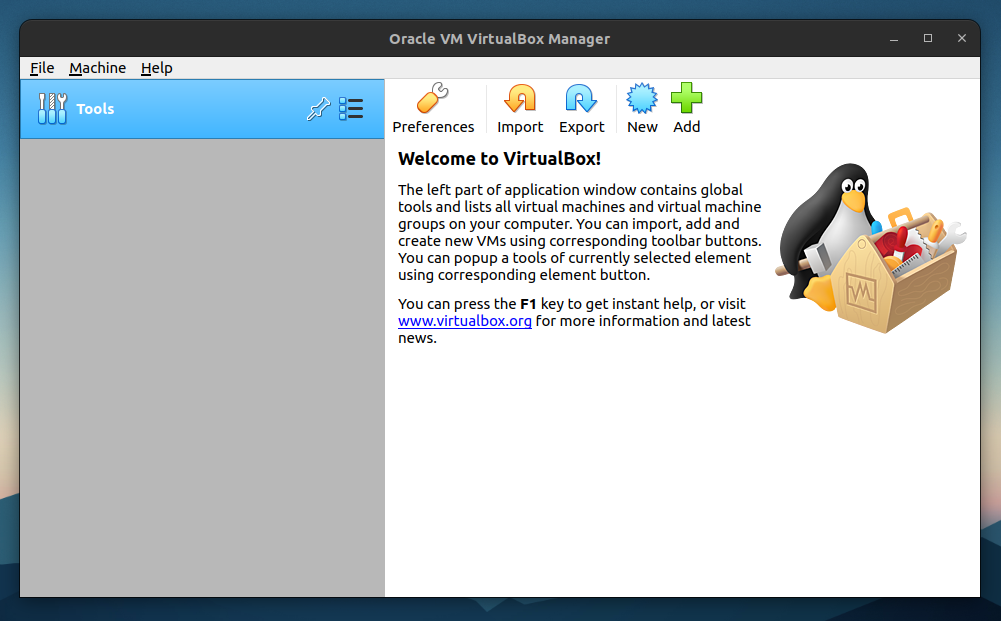
\includegraphics[scale=0.2]{img/VirtualBox.png}
  \end{center}
  Now in order to create a VM with its own OS, you need to have the appropriate \textbf{ISO file}, which is an exact copy of an entire optical disk such as a CD, DVD, or Blu-ray archived into a single file. The essentially stores the entire software needed to operate the OS. Therefore, you should download the proper ISO file from the internet (usually a couple GBs). 
  \begin{enumerate}
      \item \href{https://ubuntu.com/download/desktop}{Ubunutu ISO files}
      \item \href{https://www.microsoft.com/en-us/software-download/windows10}{Windows 10 ISO files}
      \item Apple does not allow distribution of its ISO files, so you will need to download from unofficial sources, which may be unsafe. 
  \end{enumerate}
  Once you have this ISO file, you can reuse it to create as many VMs as you want of that OS. Now follow these instructions: Click the new button and select where the virtual machine data will be stored, along with its OS. You can set the RAM, but don't make it more than half of your host computer since it will hog up too much RAM. Choose ``Create a virtual hard disk now". Choose ``VDI (VirtualBox Disk Image)". Dynamically allocated just means that the virtual disk size will adaptively grow as your storage gets full. Set the disk size to be at least 20GB. 

  After you created this, go to the VM settings (this is where you can edit your CPU cores, RAM cap, etc.). To add the ISO file, click on the ``Empty" tab right under the ``Controller:IDE", then the CD icon to the right, and ``choose a disk file". You should now choose the ISO file. Then go tweak other settings, and set the display:video memory to the max (128MB). Now you should be able to go through the installation wizard when you turn the VM on. 
  \begin{figure}[hbt!]
      \centering 
      \begin{subfigure}[b]{0.45\textwidth}
      \centering
          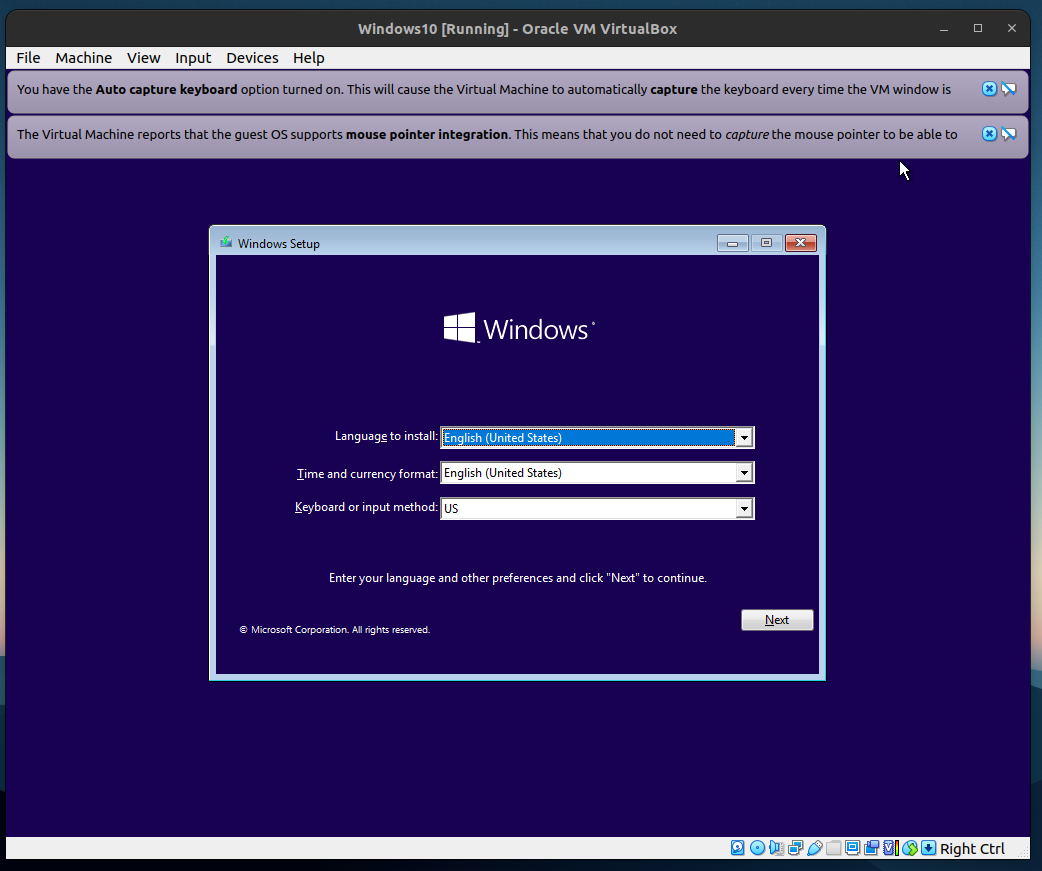
\includegraphics[width=\textwidth]{img/VM_Windows1.png}
          \caption{Windows 10 Set Up}
          \label{fig:VM_Windows1}
      \end{subfigure}
      \hfill 
      \begin{subfigure}[b]{0.45\textwidth}
      \centering
          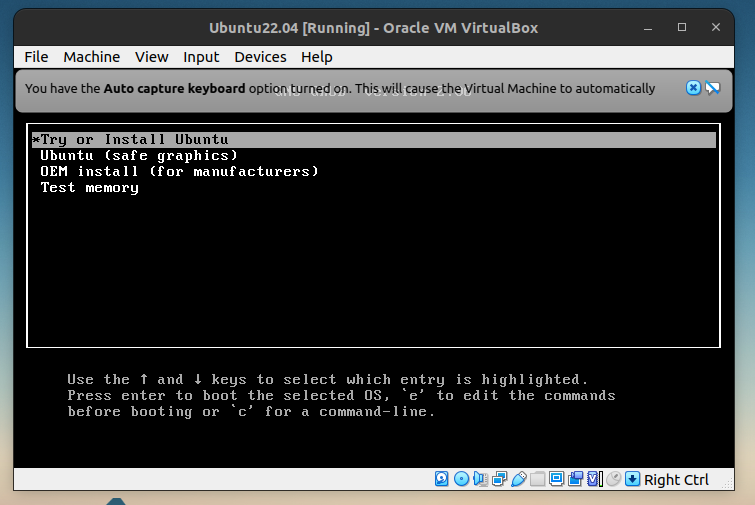
\includegraphics[width=\textwidth]{img/VM_Ubuntu1.png}
          \caption{Ubuntu 22.04 Set Up}
          \label{fig:VM_Ubuntu1}
      \end{subfigure}
      \caption{What you should get once you open up the VM after adding ISO files. }
  \end{figure}
  Refer to the instructions for each OS. 
  \begin{enumerate}
      \item For Windows: Say I don't have a product key. Click Windows 10 Home. Accept terms. Select the custom installation. Click the drive and click new, making the parititon at least 10534MB, and click apply. Next. Wait for the system to load. 
      \item For Ubuntu, you should get a GRUB view. Select ``Try or install Ubunutu". 
  \end{enumerate}
  You should now see one of these two screens. 
  \begin{figure}[hbt!]
      \centering 
      \begin{subfigure}[b]{0.45\textwidth}
      \centering
          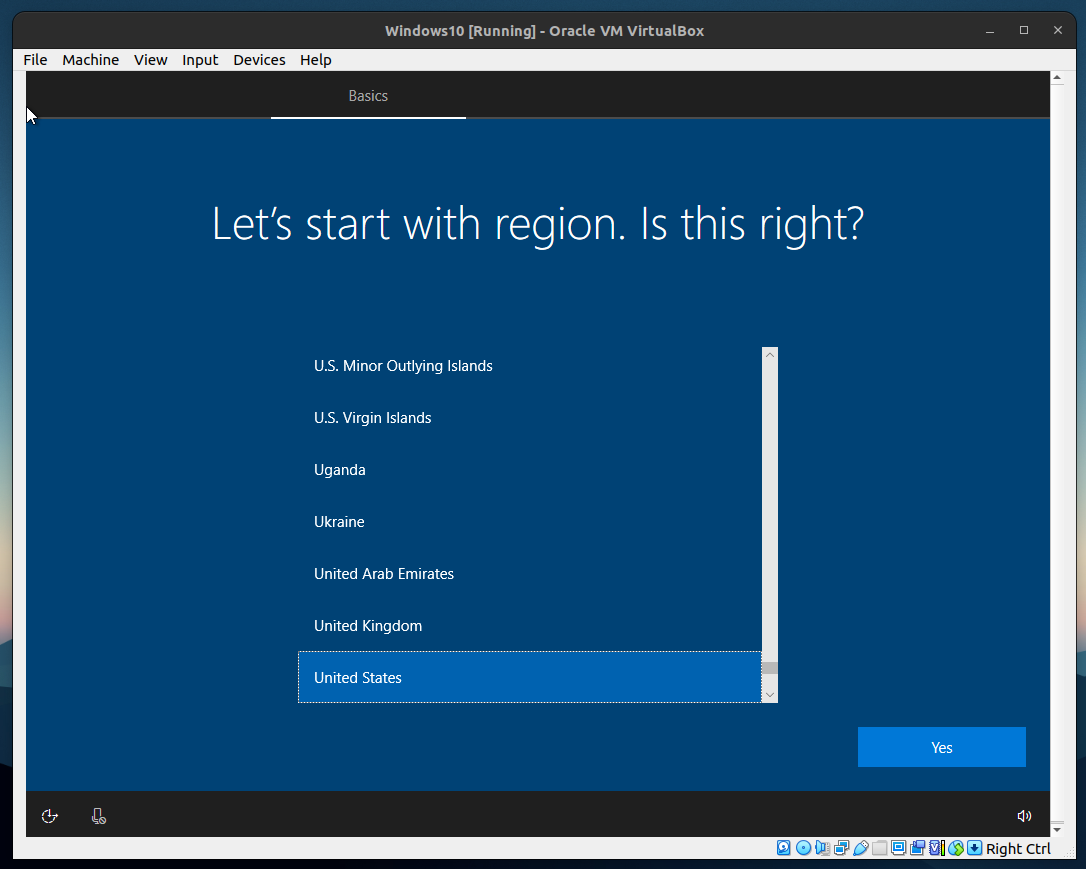
\includegraphics[width=\textwidth]{img/VM_Windows2.png}
          \caption{Windows 10 Set Up}
          \label{fig:VM_Windows2}
      \end{subfigure}
      \hfill 
      \begin{subfigure}[b]{0.45\textwidth}
      \centering
          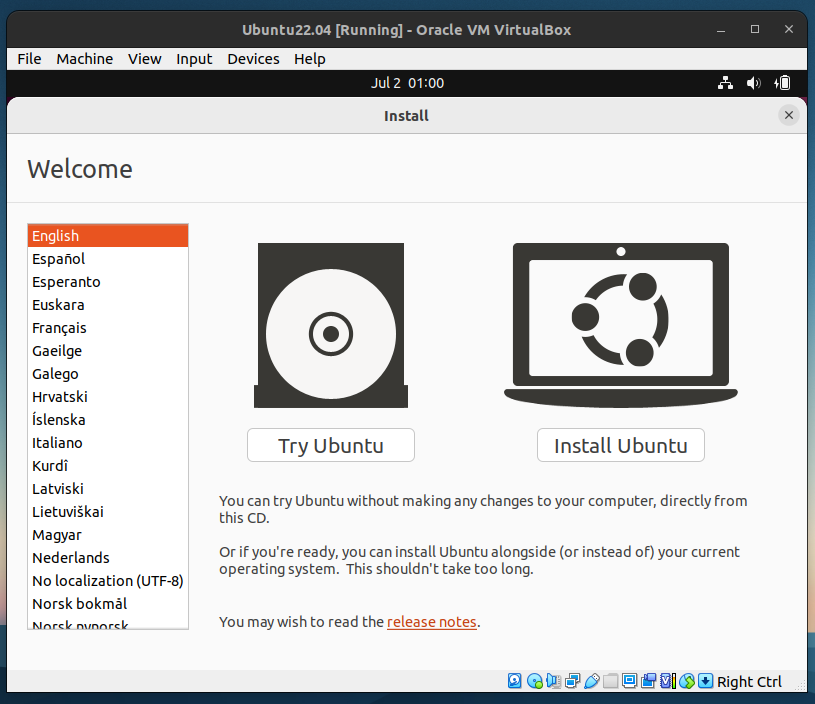
\includegraphics[width=\textwidth]{img/VM_Ubuntu2.png}
          \caption{Ubuntu 22.04 Set Up}
          \label{fig:VM_Ubuntu2}
      \end{subfigure}
      \caption{What you should get once you open up the VM after initial configuration and log in. }
  \end{figure}
  \begin{enumerate}
      \item For Windows, select your region. Select the keyboard layout. Sign in or create a Microsoft account. Choose privacy terms. Skip whatever. 
      \item For Ubuntu: Select Install Ubuntu with English. Set the keyboard layout. The normal installation may take a while, so I would select minimal depending on what you need. If you are short on time, you can uncheck the download updates while installing since you can always do that after you install. Click Erase disk and install Ubunutu. Choose region and add information. 
  \end{enumerate}
  Finally, you should see your desktop. 
  \begin{figure}[hbt!]
      \centering 
      \begin{subfigure}[b]{0.45\textwidth}
      \centering
          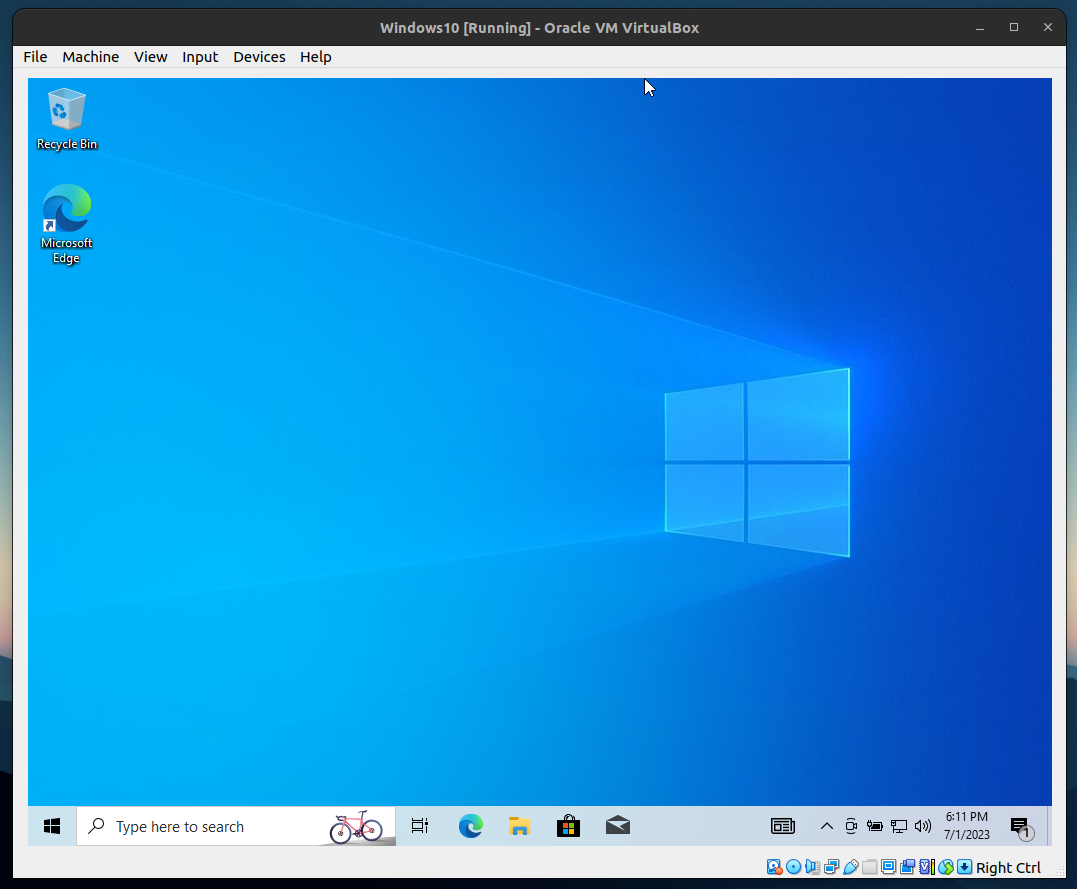
\includegraphics[width=\textwidth]{img/VM_Windows3.png}
          \caption{Windows 10 Set Up}
          \label{fig:VM_Windows3}
      \end{subfigure}
      \hfill 
      \begin{subfigure}[b]{0.45\textwidth}
      \centering
          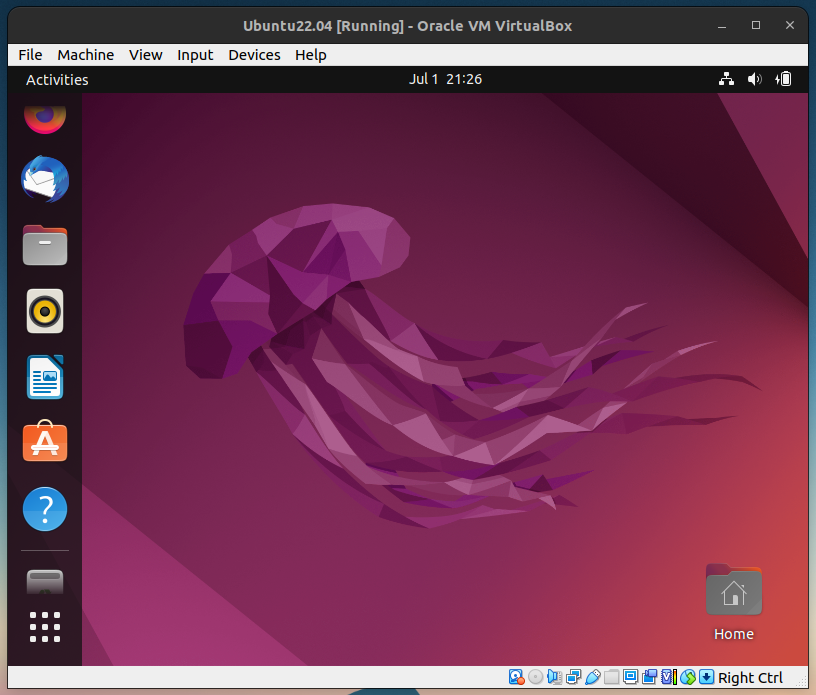
\includegraphics[width=\textwidth]{img/VM_Ubuntu3.png}
          \caption{Ubuntu 22.04 Set Up}
          \label{fig:VM_Ubuntu3}
      \end{subfigure}
      \caption{What you should see once everything is set up. }
  \end{figure}

  For my personal use, the packages below are ones that I end up installing every time I create a new VM to work in during research. 

  \begin{lstlisting}
    sudo apt update
    sudo apt install snapd
    sudo snap install --classic code
    sudo snap install slack
    sudo apt install git 
    sudo snap install spotify 
    sudo apt install htop
    wget https://dl.google.com/linux/direct/google-chrome-stable_current_amd64.deb
    sudo dpkg -i google-chrome-stable_current_amd64.deb
    sudo apt install virtualbox 
  \end{lstlisting}

  Once you are ready to use Linux consistently, it is optimal to \textbf{dual boot} it, which means that you have one computer that is divided into two: one for each operating system. Then you need to partition your drive and allocate it to your secondary OS. There are plenty of guides and tutorials online on how to do this. 

  There may be a point where you may need to resize your drive partitions as you need more or less space in one of your OS. This is when we need to do \textbf{partition resizing}. To do this, we need an empty thumb drive with at least 8GB of space in it (everything in here will be deleted). Then in your Ubuntu, install balenaEtcher and an Ubuntu (any version) ISO file. Mount the ISO file into your USB drive using balenaEtcher, following the steps in \href{https://www.youtube.com/watch?v=Kyz9x71gEPI&t=504s}{this video} to eventually get into Gparted. Another popular \href{https://www.youtube.com/watch?v=vlVXPtJ20hA&t=467s}{guide} uses Rufus in the Windows system, but I have found that this does not work for me. 

\subsection{Systemd} 

  A \textbf{process} is really any program that is running on your computer. A \textbf{daemon} is a background process that runs continuously, performing specific tasks even when no user is logged in. 

  Once the kernel has been loaded and completed its initialization process, it creates a collection of \textit{spontaneous} (as in the kernel starts them automatically) processes in user space. They're really part of the kernel implementation and don't necessarily correspond to programs in the filesystem. They're not configurable and they don't require administrative attention. These processes can be monitored with the commands \texttt{ps}, \texttt{top}, or \texttt{htop}.

  The most important process is the init process, with a system PID of 1 and with special privileges. It is used to get the system running and for starting other processes. 

  \begin{enumerate}
    \item Setting the name of the computer 
    \item Setting the time sone 
    \item Checking disks with \texttt{fsck} 
    \item Mounting filesystems 
    \item Removing old files from the \texttt{/tmp} directory 
    \item Configuring network interfaces
    \item Configuring packet filter 
    \item Starting up other daemons and network services, along with killing zombie processes or parenting orphaned processes. 
  \end{enumerate}

  There are three flavors of system management processes in widespread use: 
  \begin{enumerate}
    \item Historically, SysVinit was a series of plaintext files that ran as scripts to start processes, but due to some problems, Linux now uses systemd.
    \item An init variant that derives from the BSD UNIX, used on most BSD-based systems. 
    \item A more recent contender called \textbf{systemd} which aims to cover the init processes and much more. This significant increase in control causes some controversy. 
    \item Other flavors include Apple MacOS's \textbf{launchd} before it adopted systemd. Ubuntu also used \textbf{Upstart} before migrating to systemd. 
  \end{enumerate}

  Systemd is essentially a collection of smaller programs, services, and libraries such as systemctl, journalctl, init, process management, network management, login management, logs, etc. Some processes may depend on other processes, and with hundreds of them, it's very hard to do manually, which is why systemd does it all for you. A post on the systemd blog notes that a full build of the project generates 69 different binaries (subject to change). 

  \begin{definition}
    A \textbf{unit} is anything that is managed by systemd. It can be ``a service, a socket, a device, a mount point, an automount point, a swap file or partition, a startup carget, a watched filesystem path, a time controlled and supervised by systemd, a resource management slice, or a group of externally created processes." Within systemd, the behavior of each unit is defined and configured by a \textbf{unit file}. Within systemd, the behavior of each unit is defined and configured by a \textbf{unit file}. 

    The files are all over the place: 
      \begin{enumerate}
        \item \texttt{/lib/systemd/system} contains standard systemd unit files 
        \item \texttt{/usr/lib/systemd/system} are from locally installed packages, e.g. if I installed a pacman package that contained unit files, then those would go here. 
        \item \texttt{/etc/systemd/system} is where you put your custom files. etc also has the highest priority, so it overwrites the other files.  
        \item \texttt{/run/systemd/system} is a scratch area for transient units. 
      \end{enumerate}

    By convention, unit files are named with a suffix that varies according to the type of unit being configured. For example, service units have a \texttt{.service} suffix and timers user \texttt{.timer}. Within the unit file, some sections e.g. (\texttt{[Unit]}) apply generically to all kinds of units, but others (e.g. \texttt{[Service]}) can appear only in the context of a particular unit type. 

  \end{definition}

  \begin{example}[Service Unit File]
    If we go into one of these unit files, which have the prefix \texttt{.service}, they are usually formatted as such: 

    \begin{lstlisting}
      # comments are just the same as in bash Scripts
      # the headers are important! 

      [Unit]        #  
      Description=Description of the unit file 
      Documentation=man:something 
      After=network.target

      [Service]
      Type=forking  # tells that the process may exit and is not permanent
      PIDFile=      # 
      ExecStartPre= # scripts to run before you start 
      ExecStart=    # scripts to run when starting 
      ExecReload=   # script to run when you try to reload the process
      ExecStop=     # script to run to stop the process 

      [Install]   # Tells at what point should this be running
      WantedBy=multi-user.target 

    \end{lstlisting} 
  \end{example}
  
\subsubsection{systemctl: Managing systemd} 

  \textbf{systemctl} is an all-purpose command for investigating the status of systemd and making changes to its configuration. Running \texttt{systemctl} without any arguments invokes the default \texttt{list-units} subcommand, which shows all loaded and activive services, sockets, targets, mounts, and devices. To show only services, use \texttt{--type=service}. 

  The two main commands that you will use to interact with systemd is \texttt{systemctl} and \texttt{journalctl}. 
  
  \begin{enumerate}
    \item \texttt{systemctl status unit} checks the status, ouputting the description, whether it's enabled/disabled, and whether it's active/inactive. 
    \item \texttt{systemctl enable unit} enables it, which means that it will start when booting the computer. It does this by creating a symlink to the unit file. This is different from start. 
    \item \texttt{systemctl disable unit} disables it. 
    \item \texttt{systemctl start unit} starts it now and runs it immediately. 
    \item \texttt{systemctl stop unit} makes it inactive. 
    \item \texttt{systemctl reload} will run whatever is in the \texttt{ExecReload} in the unit file. 
    \item \texttt{systemctl restart} runs ExecStop and then ExecStart. 
    \item \texttt{systemctl kill unit} kills the process. 
  \end{enumerate}

  Some of the statuses that you may see are inactive (deactivated, exited), active (activating, running), failed, static (not started, frozen by systemd), bad (broken, probably due to bad unit files), masked (ignored by systemd), indirect (disabled, but another unit file references it so it could be activated). 

  To troubleshoot, you should run \texttt{systemctl --failed} to see if there are any failed processes, which can be a problem, and then you can use \texttt{journalctl --since=today} to view your systemd logs. This log is important for diagnosing fundamental problems with your system. To view only entries logged at the error level or above, you can set the priorities with \texttt{-p err -b}. 

\subsubsection{Targets}

\subsubsection{Systemd Logging}

  The \textbf{journald} daemon allows you to capture log messages produced by the kernel and services. These system messages are stored in the \texttt{/run} directory, but we can access them directly with the \texttt{journalctl}  command. 

  \begin{example}
    
  \end{example}

  You can configure \textbf{journald} to retain messages from prior boots. To do this, edit the following file and configure the \texttt{Storage} attribute: 
  \begin{lstlisting}
  #/etc/systemd/journald.conf
    [Journal]
    Storage=persistent
  \end{lstlisting}

  Then, you can obtain a list of prior boots with \texttt{journalctl --list-boots} and you can access messages from a prior boot by referring to its index or by naming its long-form ID: \texttt{journalctl --b -1}. 

\subsection{Directory Structure} 

  It should be clear that the $\texttt{~}$ stands for your user home directory, while $\texttt{/}$ stands for the root directory. 
  \begin{lstlisting}
  (base) mbahng@xps15:~\$ pwd
  /home/mbahng
  (base) mbahng@xps15:~\$ cd /
  (base) mbahng@xps15:/\$ pwd
  /
  \end{lstlisting}

  Let us now take a look at the contents of the root directory: 
  \begin{lstlisting}
  (base) mbahng@xps15:~\$ ls /
  bin    dev   lib    libx32      mnt   root  snap  timeshift  var
  boot   etc   lib32  lost+found  opt   run   srv   tmp
  cdrom  home  lib64  media       proc  sbin  sys   usr
  \end{lstlisting}
  You can see that the root home directory is in here, as opposed to user home directories in the $\texttt{/home}$ folder. 
  \begin{enumerate}
      \item $\texttt{root}$: This contains all the files for when you need to boot. You shouldn't mess with this. 
      \item $\texttt{etc}$: This is where you system wide configuration for applications is stored (unlike local configuration files for one user, which is stored in your home directory). It is often a target for backups. 
      \item $\texttt{media}$, $\texttt{mnt}$: Used for mounting external storage systems and even internal storage systems. 
      \item $\texttt{opt}$: A place where you can install whatever you want. Quite flexible. 
  \end{enumerate}

\subsubsection{Users and Permission}

  You should first check which users are on your system. Most people just check their home directory using 
  \begin{lstlisting}
  (base) mbahng@xps15:~\$ ls -l /home
  total 8
  drwxr-xr-x  3 root   root   4096 Jan 17 23:57 linuxbrew
  drwxr-xr-x 44 mbahng mbahng 4096 Jul  2 13:27 mbahng
  \end{lstlisting}
  But this is not accurate. Rather, we should check the contents of the $\texttt{/etc/passwd}$ file, which has a list of users in our computer (1 per line). The purpose is to contain a listing of and the options that are associated with your user accounts on your server. 
  \begin{lstlisting}
  (base) mbahng@xps15:~\$ cat /etc/passwd
  root:x:0:0:root:/root:/bin/bash
  daemon:x:1:1:daemon:/usr/sbin:/usr/sbin/nologin
  bin:x:2:2:bin:/bin:/usr/sbin/nologin
  sys:x:3:3:sys:/dev:/usr/sbin/nologin
  sync:x:4:65534:sync:/bin:/bin/sync
  games:x:5:60:games:/usr/games:/usr/sbin/nologin
  man:x:6:12:man:/var/cache/man:/usr/sbin/nologin
  lp:x:7:7:lp:/var/spool/lpd:/usr/sbin/nologin
  mail:x:8:8:mail:/var/mail:/usr/sbin/nologin
  news:x:9:9:news:/var/spool/news:/usr/sbin/nologin
  uucp:x:10:10:uucp:/var/spool/uucp:/usr/sbin/nologin
  proxy:x:13:13:proxy:/bin:/usr/sbin/nologin
  www-data:x:33:33:www-data:/var/www:/usr/sbin/nologin
  backup:x:34:34:backup:/var/backups:/usr/sbin/nologin
  list:x:38:38:Mailing List Manager:/var/list:/usr/sbin/nologin
  irc:x:39:39:ircd:/run/ircd:/usr/sbin/nologin
  gnats:x:41:41:Gnats Bug-Reporting System (admin):/var/lib/gnats:/usr/sbin/nologin
  nobody:x:65534:65534:nobody:/nonexistent:/usr/sbin/nologin
  ...
  \end{lstlisting}
  Let us just examine my user. 
  \begin{lstlisting}
  (base) mbahng@xps15:~\$ cat /etc/passwd | grep mbahng
  mbahng:x:1000:1000:mbahng,,,:/home/mbahng:/bin/bash
  \end{lstlisting}
  Going from left to right, mbahng is my user, the x stands for a hashed password that cannot be shown, the 1000 is the user id (UID), the 1000 is the group id (GID), mbahng is the user information field (optional), next $\texttt{/home/mbahng}$ is the user's home directory, and finally $\texttt{/bin/bash}$ is the shell designated for the user. When you create a user id when first installing Ubuntu, this will almost always have uid of 1000. On most linux distributions, the user accounts that will be used by humans are given uids of 1000 and above. Note that in Ubunutu 22.04, a home directory is not created automatically (this differs based on distribution) when we create a new user. So note the following commands. To add a user called batman, we have 
  \begin{lstlisting}
  (base) mbahng@xps15:~\$ sudo useradd batman         # just add user 
  (base) mbahng@xps15:~\$ sudo useradd -m batman      # add user with home dir 
  (base) mbahng@xps15:~\$ cat /etc/passwd | grep batman
  batman:x:1001:1001::/home/batman:/bin/sh
  \end{lstlisting}
  and it gives a new uid that is the next available one from 1000, i.e. 1001. To delete the user, just do 
  \begin{lstlisting}
  (base) mbahng@xps15:~\$ sudo userdel batman         # delete user
  (base) mbahng@xps15:~\$ sudo userdel -r batman      # delete user w/ home dir
  \end{lstlisting}
  Now let's talk about changing passwords. If you want to change your own password, you can just type $\texttt{passwd}$ and go through the steps. To set another user's password, you need to be in root mode and type 
  \begin{lstlisting}
  (base) mbahng@xps15:~\$ sudo passwd batman          # set password for batman
  \end{lstlisting}

  Note that we have a hashed version of the user's password in the $\texttt{/etc/passwd}$ file. We can actually see the full hashed versions by going into $\texttt{/etc/shadow}$. 

  Running $\texttt{ls -l}$ command lists all files and directories in your current working directory, along with their permissions. 
  \begin{lstlisting}
    -rw-rw-r--  1 mbahng mbahng 4336730777 Sep 29  2022  cuda_11.8.0_520.61.05_linux.run
    drwxr-xr-x  9 mbahng mbahng       4096 Jul  1 23:33  Desktop
    drwxr-xr-x  8 mbahng mbahng       4096 Jul  1 15:08  Documents
    drwxr-xr-x  6 mbahng mbahng      12288 Jul  1 22:36  Downloads
    drwxr-xr-x  4 mbahng mbahng       4096 Jun 29 19:43  Games
    drwxr-xr-x  6 mbahng mbahng       4096 Feb 22 17:27  Jts
    drwxrwxr-x  5 mbahng mbahng       4096 Jun 28 19:39  KakaoTalk
    drwxr-xr-x 16 mbahng mbahng       4096 Jun  2 21:13  miniconda3
    drwxrwxr-x  4 mbahng mbahng       4096 Jun 22 13:12  nltk_data
  \end{lstlisting}
  The first columm is a string of 10 characters representing the permissions. They are divided into 4 sections: 
  \begin{lstlisting}
  d   rwx   r-x   r-x 
  \end{lstlisting}
  The first letter can be a d, l, or -, meaning directory, link, or file, respectively. The next three groups, representing the permissions of the user (third columm), group (fourth), and everyone else, have the same format. It is rwx, which stands for read, write, execute. 
  \begin{enumerate}
      \item Read: Means to read a file or read a directory. 
      \item Write: Means to edit a file or modify the contents of a directory. 
      \item Execute: Means to run the file as an executable or go $\texttt{cd}$ into the directory. 
  \end{enumerate}
  A dash in place of any one of them means that whatever entity does not have the permissions. However, we can set the permissions using the $\texttt{chmod}$ command. If we have a file named $\texttt{testfile.txt}$ in our current directory, we can add or revoke permissions with 
  \begin{lstlisting}
  chmod +r testfile.txt   // assign read permissions to all users
  chmod +w testfile.txt   // assign write permissions to all users
  chmod +x testfile.txt   // assign execute permissions to all users

  chmod g+rw testfile.txt   // assign read and write to group 
  chmod u-r testfile.txt   // revoke read to user
  chmod o+x testfile.txt   // assign execute to other users 
  \end{lstlisting} 
  Writing all these can be tedious, so what we can do is take advantage of the numerical encodings of the permissions. Note that $r=4, w=2, x=1$, and so any number between $0$ and $7$ can encode the three bits (through the coefficients of the binary expansion). Therefore, if we wanted every permission for all users, we can write 
  \begin{lstlisting}
  chmod 770 testfile.txt
  \end{lstlisting}
  where the first 7 stands for $\texttt{rwx}$, the next 7 stands for $\texttt{rwx}$, and the final $0$ stands for $\texttt{---}$. To change the permissions for everything inside a directory (e.g. say you want to make all downloads only readable and writable by you), then you can type 
  \begin{lstlisting}
  chmod 600 ~/Downloads/*
  \end{lstlisting}

  If you have multiple users in your computer (type $\texttt{ls /home}$), then you may want to give ownership of a directory or folder to another user. 
  \begin{lstlisting}
    (base) mbahng@xps15: ls /home
    batman mbahng
  \end{lstlisting}
  To change permissions of a file/directory to another user and group, we can use the $\texttt{chown}$ command (with sudo) 
  \begin{lstlisting}
    sudo chown -R batman:batman Downloads/
  \end{lstlisting}

\subsection{Display Servers}

  When you boot up your computer, you are greeted with a graphical user interface (GUI) that allows you to interact with your computer. This is the job of the display server, which is a program that provides graphical display capabilities for the operating system. 

  \begin{definition}[Display Server]
    A \textbf{display server} is a program that manages the communication between your computer's hardware and graphical software applications. It acts as a bridge for input and output devices; for example, it processes the input from your keyboard and mouse and outputs graphics to the monitor. The display server is responsible for the fundamental task of drawing windows and handling the low-level aspects of input and output, but it doesn't dictate how these windows look or are arranged. For almost every purpose, there are two types of display servers: 
    \begin{enumerate} 
      \item \textbf{X}: The X Window System, which is the older and more established display server. 
      \item \textbf{Wayland}: The newer and more modern display server.
    \end{enumerate}
  \end{definition}

  \begin{definition}[X Window System]
    The \textbf{X Window System} is a windowing protocol for Unix/Linux OSes, similar to the way that Microsoft Windows or Apple Mac OS X can run different apps in separate windows. \textbf{X} defines the protocol for a display server what can render windows on a \textit{display client} (your computer), inside which are running apps.\footnote{Explanation here: https://www.reddit.com/r/linuxquestions/comments/3uh9n9/what\_exactly\_is\_xxorgx11/} 
    \begin{enumerate} 
      \item \textbf{X11} refers to version 11 of the X protocol, while 
      \item \textbf{Xorg} is an open-source implementation of X. 
    \end{enumerate}
  \end{definition}

  \begin{definition}[Wayland]
    X, made in 1984, has developed a lot of cruft over the years, and Wayland is a modern replacement for X. It is a protocol for a compositor to talk to its clients, as well as a C library implementation of that protocol. The compositor can be a standalone display server running on Linux kernel modesetting and evdev input devices, an X application, or a wayland client itself. 
  \end{definition}

\subsection{Package Management}
  
  Linux comes in many flavors of distributions. Most beginners look at screenshots of these distributions on the internet and judge them based on their aesthetics (e.g. I like how Kali Linux looks so I'll go with that one). A common feature of all Linux distributions is that they provide the user the power to customize their system however they want, so you can essentially make every linux distribution look like any other. So what are some things you should consider when choosing a distribution? 

  \begin{enumerate}
    \item First is the popularity and how well it is supported. This includes the number of people who use the distribution (e.g. the Ubuntu StackExchange is a very large community) and how good the documentation is overall (e.g. the ArchLinux wiki is very well documented). 
    \item Each linux distribution essentially consists of a kernel and package manager. The architecture, design, and the update scheme of the kernel may be an interest to many linux users.  
    \item Every distribution has its own native package manager, and the availability of certain necessary packages, the ease of installation, and the updating schemes is also something to consider.  
    \item The ideals of the respective communities. The community behind each distribution has a certain set of ideals that they lean more towards. For example, the Ubuntu community likes having programs that are right out of the box, with good GUI support and is more beginner-friendly while Arch has more of a minimal and extremely customizable nature to it with its software being much more CLI dependent. 
  \end{enumerate}

  Let's begin with the package managers. Every application on your system (Firefox, Spotify, pdf readers, VSCode, etc.) is a package, and manually downloading and managing each one is impossible to do. Therefore, each distribution has its own native package manager that automatically takes care of downloading, installing, removing, checking dependency requirements of each package. In order to download a package, a package manager should also know where it is downloading \textit{from}. Essentially, a package manager itself can be downloaded with other package managers, so package managers are packages as well. 
  
  \begin{enumerate}
    \item \textbf{apt} : The advanced packaging tool is the native manager for Ubuntu distributions. 
    \item \textbf{pacman} : Native package manager for Arch Linux. 
    \item \textbf{yay} : The package manager for software in the \textbf{Arch User Repository}. 
    \item \textbf{snap} : 
    \item \textbf{flatpak} : 
    \item \textbf{dpkg} : Package manager for Debian based distributions. 
  \end{enumerate}

  Chances are if you are using one distribution, you would only have to work with a small subset of these package managers. Each package manager has one or more files in the computer that specify a list of \textbf{repositories}. 

  \subsection{Wget}

    wget is a command-line utility used to download files from the internet. It stands for "web get." 

  \subsection{Pacman}

    For example, the configuration file for pacman is located at \texttt{/etc/pacman.conf}. In the options section, I can configure stuff like text color, enabling/disabling parallel downloads, choosing specific packages to ignore upgrading, etc. Then, we can specify the servers that we should download from. In the text below, the server variable defines which server we should look at first, and then the Include variable stores the location of the file \texttt{mirrorlist} that defines a list of other servers that we should download from. 
    
    \begin{figure}
      \begin{lstlisting} 
        # The following paths are commented out with their default values listed.
        # If you wish to use different paths, uncomment and update the paths.
        #RootDir     = /
        #DBPath      = /var/lib/pacman/
        #CacheDir    = /var/cache/pacman/pkg/
        #LogFile     = /var/log/pacman.log
        #GPGDir      = /etc/pacman.d/gnupg/
        #HookDir     = /etc/pacman.d/hooks/
        HoldPkg     = pacman glibc
        #XferCommand = /usr/bin/curl -L -C - -f -o %o %u
        #XferCommand = /usr/bin/wget --passive-ftp -c -O %o %u
        #CleanMethod = KeepInstalled
        Architecture = auto

        # Pacman won't upgrade packages listed in IgnorePkg and members of IgnoreGroup
        #IgnorePkg   =
        #IgnoreGroup =

        #NoUpgrade   =
        #NoExtract   =

        # Misc options
        #UseSyslog
        #Color
        #NoProgressBar
        CheckSpace
        #VerbosePkgLists
        ParallelDownloads = 5
        ILoveCandy

      \end{lstlisting}
      \caption{Subset of contents of the \texttt{/etc/pacman.conf} file} \label{fig:pacman.conf}
    \end{figure}
    
    The mirrorlist file stores a list of URLs. Each URL is a \textbf{mirror}, which is a server that contains a physical replica of all the packages that are available to you via \texttt{pacman} (hence the name mirror). You can literally type in the links provided in Figure \ref{fig:mirrorlist} (replacing \texttt{\$repo} with \texttt{core} and \texttt{\$arch} with \texttt{x86\_64}). It contains a tarball of each package ready to be downloaded. Some repos might contain more packages than others, some might have packages that only they supply that others don’t, but if you can install the piece of software via your package manager then one of your configured repos is declaring they have it available and therefore should have the file on hand to give to you if asked for it. A list of all available mirrors are available \href{https://archlinux.org/mirrorlist/all/https/}{here} (this only uses HTTPS, but HTTP mirrors are also available).  

    \begin{figure}
      \begin{lstlisting}
        Server = https://archlinux.mailtunnel.eu/$repo/os/$arch
        Server = https://mirror.cyberbits.eu/archlinux/$repo/os/$arch
        Server = https://mirror.theo546.fr/archlinux/$repo/os/$arch
        Server = https://mirror.sunred.org/archlinux/$repo/os/$arch
        Server = https://mirror.f4st.host/archlinux/$repo/os/$arch
        Server = https://md.mirrors.hacktegic.com/archlinux/$repo/os/$arch
        Server = https://mirrors.neusoft.edu.cn/archlinux/$repo/os/$arch
        Server = https://mirror.moson.org/arch/$repo/os/$arch
        Server = https://archlinux.thaller.ws/$repo/os/$arch
      \end{lstlisting}
      \caption{Contents of the \texttt{/etc/pacman.d/mirrorlist} file}\label{fig:mirrorlist}
    \end{figure}
    
    The mirrors that you download from should be trustworthy and fast. The speed is mainly related to how close you are to that mirror geographically, so if you are moving to another country you should probably update this mirrorlist for faster download speeds. There is a default mirrorlist file that is generated, but you can download and use the \textbf{reflector} package to update it.  

    Here are some common commands: 
    \begin{enumerate}
      \item Install a package: \texttt{sudo pacman -S pkg1} (\texttt{-s} stands for synchronize)

      \item Remove a package: \texttt{sudo pacman -R pkg}
      \begin{itemize}
        \item remove dependencies also: \texttt{-s} (recursive)
        \item also remove configuration files: \texttt{-n} (no save)
        \item also removes children packages: \texttt{-c} (cascade)
      \end{itemize}

      \item Update all packages: \texttt{sudo pacman -Syu}
      \begin{itemize}
        \item synchronize: \texttt{-S}
        \item refresh package databases: \texttt{-y} (completely refresh: \texttt{-yy})
        \item system upgrade: \texttt{-u}
      \end{itemize}

      \item List installed packages: \texttt{pacman -Q}
      \begin{itemize}
        \item List detailed info about a package: \texttt{pacman -Qi pkg}
        \item List all files provided by a package: \texttt{pacman -Ql pkg}
        \item List all orphaned packages: \texttt{pacman -Qdt}
        \item List all packages that have updates available: \texttt{pacman -Qu}
        \item List all explicitly installed packages: \texttt{pacman -Qet}
        \item Display the dependency tree of a package: \texttt{pactree pkg} (from the \texttt{pacman-contrib} package) 
        \item List last 20 installed packages: 
        \begin{lstlisting}
          expac --timefmt='%Y-%m-%d %T' '%l\t%n' | sort | tail -n 20
        \end{lstlisting}
      \end{itemize}

      \item To check size of current packages and dependencies, download \texttt{expac} and run \texttt{expac -H M '\%m \\t\%n' | sort -h} 

      \item The package cache stored in \texttt{/var/cache/pacman/pkg/} keeps old or uninstalled versions of packages automatically. This is helpful since it also keeps older versions of packages in the cache, and you can manually downgrade in case some packages break.  
      \begin{itemize}
        \item We can delete all cached versions of installed and uninstalled packages, except for the most recent 3, by running \texttt{paccache -r} (provided by the \texttt{pacman-contrib} package). 
        \item To remove all cached packages not currently installed, run \texttt{pacman -Sc}
        \item To remove all cached aggressively, run \texttt{pacman -Scc}
        \item To downgrade, you go into the package cache directory and say you want to see which versions of neovim you have installed. You can \texttt{ls} the directory to see the following. 
        
          \begin{lstlisting}
            neovim-0.9.5-1-x86_64.pkg.tar.zst
            neovim-0.9.5-1-x86_64.pkg.tar.zst.sig
            neovim-0.9.5-2-x86_64.pkg.tar.zst
            neovim-0.9.5-2-x86_64.pkg.tar.zst.sig
          \end{lstlisting}

          We have an older version of neovim installed, and to roll it back we can use 
          \begin{lstlisting} 
            pacman -U neovim-0.9.5-1-x86_64.pkg.tar.zst
          \end{lstlisting}
      \end{itemize} 
    \end{enumerate}

    The pacman log (\texttt{/var/log/pacman.log}) is also useful since it logs all pacman outputs when you do anything with pacman. So if you are looking for the packages that have been installed in the latest \texttt{pacman -Syu}, then you can use this to individually see each package that has been upgraded. 

  \subsection{Yay}

    Yay is used to install from the Arch User repository and must be updated separately. To run this, you can either run \texttt{yay -Syu} or you can just run \texttt{yay}. Since this is not officially maintained, these packages are more likely to break something. The yay logs are not stored separately can can be accessed in the pacman logs. 

  \subsection{Dpkg and Deb files}

    Ubuntu is a Linux distribution within the family of Debian-based systems (with Debian, Linux Mint, etc.). File of the $\texttt{.deb}$ format is used to distribute and install software packages on these systems. A deb package contains the files for a particular software application or library, along with metadata that describes the package and instructions on how to install or remove it. The package format follows a specific structure and includes files such as control files, data files, and scripts. Therefore, many downloaded packages may come in this format, similar to how a file is zipped before we have to extract it. 

    Dpkg is the primary package manager for Debian based systems. It installs, builds, removes, configures, and retrieves information for Debian packages of the $\texttt{.deb}$ format. Given that we have some file $\texttt{package.deb}$ downloaded, the command 
    \begin{lstlisting}
      dpkg -i package.deb
    \end{lstlisting}
    installs the specified package from the $\texttt{package.deb}$ file. Removing it is just (note without the suffix) 
    \begin{lstlisting}
      dpkg -r package
    \end{lstlisting}

  \subsection{Apt}

    \href{https://www.reddit.com/r/Ubuntu/comments/9awvip/eli5_snap_and_flatpak_how_are_they_differ_from_apt/}{read more here}

    While dpkg is the native package manager for Debian based systems, apt is just a built-in Ubuntu tool to help install these Debian packages and manage dependencies. To run apt commands, we must have root privilege, so we should always use sudo. When these command are run, you should get a confirmation question asking whether you want to continue, with [Y/n]. The capital letter is the default, so you can either enter in `y' or just press ENTER. 
    \begin{enumerate}
      \item The update command connects to various URLs to download a list of available packages. Periodically, new packages are introduced to Debian and Ubunutu repositories all the time, so this command refreshes the index so that it knows what packages are available and at what versions. It is a good idea to run this before you use apt commands for the day. 
      \begin{lstlisting}
        sudo apt update
      \end{lstlisting}

      \item The upgrade command just updates all packages and their dependencies to their latest versions. However, this does not update packages which require the installation of \textit{additional} packages. 
      \begin{lstlisting}
        sudo apt upgrade 
      \end{lstlisting}

      \item The dist upgrade updates packages including those that need installation of new dependencies. So it is a good idea to run upgrade first and then dist-upgrade after.  
      \begin{lstlisting}
        sudo apt dist-upgrade 
      \end{lstlisting}
    \end{enumerate}

    Installing and removing packages is easy. 

    \begin{enumerate}
      \item We can install from the apt repository with 
      \begin{lstlisting}
        sudo apt install htop
      \end{lstlisting}

      \item We can remove it with 
      \begin{lstlisting}
        sudo apt remove htop
      \end{lstlisting}
    \end{enumerate}

    If you don't know the name of the application or package you want to install, then you can search for a keyword with apt search. Say that you want to install vim but you don't know what the actual package name is called. You can just type 

    \begin{lstlisting}
      apt search vim
    \end{lstlisting}

    The central location where apt gets its updates from is contained in the $\texttt{/etc/apt/sources.list}$ file. Here is a snippet of it in my system. 
    \begin{lstlisting}
      # deb cdrom:[Ubuntu 22.04.1 LTS _Jammy Jellyfish_ - Release amd64 (20220809.1)]/ 
      jammy main restricted

      # See http://help.ubuntu.com/community/UpgradeNotes for how to upgrade to
      # newer versions of the distribution.
      deb http://us.archive.ubuntu.com/ubuntu/ jammy main restricted
      # deb-src http://kr.archive.ubuntu.com/ubuntu/ jammy main restricted

      ## Major bug fix updates produced after the final release of the
      ## distribution.
      deb http://us.archive.ubuntu.com/ubuntu/ jammy-updates main restricted
      # deb-src http://kr.archive.ubuntu.com/ubuntu/ jammy-updates main restricted

      ## N.B. software from this repository is ENTIRELY UNSUPPORTED by the Ubuntu
      ## team. Also, please note that software in universe WILL NOT receive any
      ## review or updates from the Ubuntu security team.
      deb http://us.archive.ubuntu.com/ubuntu/ jammy universe
      # deb-src http://kr.archive.ubuntu.com/ubuntu/ jammy universe
      deb http://us.archive.ubuntu.com/ubuntu/ jammy-updates universe
      # deb-src http://kr.archive.ubuntu.com/ubuntu/ jammy-updates universe
      ...
    \end{lstlisting}

  \subsection{Snap and Flatpak}

    Other package managers that you may need to use often are snap and flatpak, which can both be installed with 
    \begin{lstlisting}
      sudo apt install snap flatpak 
    \end{lstlisting}

\subsection{Windows Managers and Desktop Environments}

  These days, the terms window managers (WMs) and Desktop Environments (DEs) are used interchangeably, but they mean slightly different things. A window manager is the display software that determines how the pixels for each window overlaps with other and their movement. This is generally divided into two paradigms with the most familiar being \textbf{floating WMs} and the other being \textbf{tiling WMs}. Even before I knew about tiling WMs, I found myself manually tiling windows on floating WMs, so the move to tiling WMs was a no-brainer. 
  
  Some DEs and WMs are: 
  \begin{enumerate}
    \item GNOME 
    \item KDE Plasma
    \item Qtile
  \end{enumerate}

\subsection{Shells and Terminals}

  Beginners may think of the shell and the terminal to be the same thing, but they are different. The \textbf{shell} is a command line interpreter, a layer that sits on top of the kernel in which the user can interact with. It is essentially the only API to the kernel where the user can input commands and processes them. The \textbf{terminal emulator} is a wrapper program that runs a shell and allows us to access the API. It may be useful to think of the shell as like a programming language and the terminal as a text editor like VSCode. 

  The three most common shells are the following: 
  \begin{enumerate}
    \item \textbf{Bash}: 
    \item \textbf{Zsh}: 
    \item \textbf{Fish}:  
  \end{enumerate}

  Some common terminal emulators (most of which comes as a part of the desktop environment) are the following: 
  \begin{enumerate}
    \item \textbf{Kitty}: 
    \item \textbf{Alacritty}: 
    \item \textbf{Gnome-Terminal}: 
  \end{enumerate}

\subsubsection{Crontab}

  To schedule jobs, you run $\texttt{crontab -e}$, which will give you a text file for which you can list jobs. It looks like  

  \begin{lstlisting}
    # Edit this file to introduce tasks to be run by cron.
    # 
    # Each task to run has to be defined through a single line
    # indicating with different fields when the task will be run
    # and what command to run for the task
    # 
    # To define the time you can provide concrete values for
    # minute (m), hour (h), day of month (dom), month (mon),
    # and day of week (dow) or use '*' in these fields (for 'any').
    # 
    # Notice that tasks will be started based on the cron's system
    # daemon's notion of time and timezones.
    # 
    # Output of the crontab jobs (including errors) is sent through
    # email to the user the crontab file belongs to (unless redirected).
    # 
    # For example, you can run a backup of all your user accounts
    # at 5 a.m every week with:
    # 0 5 * * 1 tar -zcf /var/backups/home.tgz /home/
    # 
    # For more information see the manual pages of crontab(5) and cron(8)
    # 
    # m h  dom mon dow   command
  \end{lstlisting}

  In the bottom line, we can add the following to run $\texttt{sudo apt update}$ every minute. The 5 columns refer to minute (0-59), hour (0-24), date of month (1-31), month (1-12), and date of week (0-7, where 0 and 7 is Sunday). The asterick means every instance of. 

  \begin{lstlisting}
    # Run every minute
    * * * * * sudo apt update 

    # Run at 9:15am every first day of the month 
    15 9 1 * * sudo apt update

    # Run for every minute of every hour for the 13th day of every month if it is Friday
    * * 13 * 5 sudo apt update
  \end{lstlisting}
  You get the idea. 

\subsection{Graphics Drivers}
  
  Note that one type of data we must store on memory is the individual pixels in a computer screen. Say that in a $1920 \times 1080$ resolution computer, there are about $1920 \times 1080 \times 3 \approx 2$ million bytes of data that we have to store. This isn't that much data (only 2MB), but we must update it quite fast since our screens are always updating. This is why all computer which have a GUI comes with a built-in graphics driver. To see the GPU hardware specifications, install \textbf{lshw}. 

  \begin{definition}[Graphics Processing Unit]
    The \textbf{GPU} is a specialized processing unit that is designed to handle the rendering of images and videos. It is designed to handle the rendering of images and videos, and is optimized for parallel processing. Like the CPU, it has some common metrics: 
    \begin{enumerate} 
      \item \textbf{Clock Speed}: The speed at which the GPU can execute instructions. This is usually measured in MHz or GHz. 
      \item \textbf{Memory}: The amount of memory that the GPU has. This is usually measured in GB. 
      \item \textbf{Memory Bandwidth}: The speed at which the GPU can read and write to its memory. This is usually measured in GB/s. 
      \item \textbf{Cores}: The number of cores that the GPU has. This is usually measured in thousands, which allows for parallel processing. 
    \end{enumerate}
    You can check which GPUs you have by running \texttt{lspci | grep VGA} or \texttt{neofetch}. There are generally two types of GPUs: 
    \begin{enumerate} 
      \item \textbf{Integrated GPU}: This type of GPU is built into the same chip as the CPU (Central Processing Unit). It shares resources with the CPU, including memory, which can lead to reduced performance for graphics-intensive tasks. However, its integrated nature makes it more power-efficient and cost-effective. 
      \item \textbf{Discrete GPU}: This is a separate component from the CPU and comes with its own RAM (usually called VRAM or Video RAM). It is typically installed in a dedicated slot on the motherboard. Because it operates independently of the CPU, a discrete GPU can offer significantly better performance for graphics processing, gaming, or deep learning. 
    \end{enumerate}
  \end{definition}

  \begin{definition}[Monitor]
    Furthermore, your computer monitor, which actually displays these pixels to you, must also have metrics that match the GPU. Some properties: 
    \begin{enumerate} 
      \item The \textbf{resolution} is the number of pixels that the monitor can display, and is usually measured in pixels. 
      \item The \textbf{refresh rate} is the number of times the monitor can refresh the image on the screen per second, and is usually measured in Hz. 
    \end{enumerate}
    To see these metrics for all monitors connected to your computer, run \textbf{xrandr}, which lists all the resolutions and possible refresh rates for each resolution. 
  \end{definition}

  \begin{definition}[Graphics Driver]
    In order for your operating system to communicate with your GPU, you need a \textbf{graphics driver}. This is a piece of software that allows the operating system to communicate with the GPU. There are two main types of graphics drivers:
    \begin{enumerate} 
      \item \textbf{Open Source Drivers}: These are drivers that are developed and maintained by the open source community. They are usually included with the Linux kernel, and are generally stable and reliable. 
      \item \textbf{Proprietary Drivers}: These are drivers that are developed and maintained by the GPU manufacturer. They are usually not included with the Linux kernel, and are generally more feature-rich and performant than open source drivers. 
    \end{enumerate}
  Intel drivers are open source, but Nvidia drivers are proprietary (which is why Linus Torvalds has beef with Nvidia).\footnote{A video of Linus Torvalds saying ``fuck you'' to Nvidia: https://www.youtube.com/watch?v=iYWzMvlj2RQ}
  \end{definition}

  Some popular graphics drivers include \textbf{mesa} for Intel and \textbf{nvidia} drivers for NVIDIA. 

  \subsubsection{Multiple GPUs} 

    Everything is pretty straightforward when you have one graphics card, but when you have multiple graphics cards, you have to specify which one you want to use. If you want to only use one GPU, you can just disable the other one in the BIOS. However, if you have an Intel/Nvidia dual driver and want to use both, install \textbf{Nvidia Optimius} (for Ubuntu, it is supported through \textbf{nvidia-prime}).\footnote{This wiki article (https://github.com/Askannz/optimus-manager/wiki) provides a good overview of this matter. },\footnote{Installation instructions here: https://github.com/Askannz/optimus-manager?tab=readme-ov-file} 

    Now make sure that the systemd daemon is running, and you can call \texttt{optimus-manager --switch hybrid} to enable hybrid graphics. This will log you out. 

  \subsection{Peripheral Devices} 
    
    Peripheral devices refer to other devices outside of the motherboard, including mice, keyboards for input, monitors, printers, network managers, and usb ports. Even the GPU is considered a peripheral device. These must be connected to the motherboard in some way to be managed by the operating system, and similar to the databus connecting the CPU and memory, there are buses that connect the motherboard and these peripheral devices. 

    \begin{definition}[PCI Bus]
      The \textbf{PCI (Peripheral Component Interconnect)} bus is a high-speed bus that connects the motherboard to peripheral devices. It is used to connect devices like network cards, sound cards, and graphics cards to the motherboard. PCI buses operated based on the PCI standard, which is a set of specifications that define the physical and electrical characteristics of the bus. 
    \end{definition}

    The command to use to enumerate all PCI devices is \texttt{sudo lspci} (with \texttt{-v} for verbose). 
    
    \begin{figure}[hbt!]
      \centering 
      \begin{lstlisting} 
        00:00.0 Host bridge: Intel Corporation 10th Gen Core Processor 
        00:01.0 PCI bridge: Intel Corporation 6th-10th Gen Core Processor 
        00:02.0 VGA compatible controller: Intel Corporation CometLake-H 
        00:04.0 Signal processing controller: Intel Corporation Xeon 
        00:08.0 System peripheral: Intel Corporation Xeon E3-1200 v5/v6 
        00:12.0 Signal processing controller: Intel Corporation Comet 
        00:13.0 Serial controller: Intel Corporation Device 06fc
        00:14.0 USB controller: Intel Corporation Comet Lake USB 3.1 
        00:14.2 RAM memory: Intel Corporation Comet Lake PCH Shared 
        00:14.3 Network controller: Intel Corporation Comet Lake PCH
        00:15.0 Serial bus controller: Intel Corporation Comet Lake 
        00:15.1 Serial bus controller: Intel Corporation Comet Lake 
        00:16.0 Communication controller: Intel Corporation Comet 
        00:1c.0 PCI bridge: Intel Corporation Device 06b8 (rev f0)
        00:1c.6 PCI bridge: Intel Corporation Device 06be (rev f0)
        00:1d.0 PCI bridge: Intel Corporation Comet Lake PCI Express
        00:1e.0 Communication controller: Intel Corporation Comet Lake 
        00:1f.0 ISA bridge: Intel Corporation Device 068e
        00:1f.3 Audio device: Intel Corporation Comet Lake PCH cAVS
        00:1f.4 SMBus: Intel Corporation Comet Lake PCH SMBus Controller
        00:1f.5 Serial bus controller: Intel Corporation Comet Lake 
        01:00.0 3D controller: NVIDIA Corporation TU117M [GeForce GTX 1650 
        02:00.0 PCI bridge: Intel Corporation JHL7540 Thunderbolt 3 Bridge
        03:00.0 PCI bridge: Intel Corporation JHL7540 Thunderbolt 3 Bridge
        03:01.0 PCI bridge: Intel Corporation JHL7540 Thunderbolt 3 Bridge
        03:02.0 PCI bridge: Intel Corporation JHL7540 Thunderbolt 3 Bridge
        03:04.0 PCI bridge: Intel Corporation JHL7540 Thunderbolt 3 Bridge
        04:00.0 System peripheral: Intel Corporation JHL7540 Thunderbolt 
        38:00.0 USB controller: Intel Corporation JHL7540 Thunderbolt 3 
        6c:00.0 Unassigned class [ff00]: Realtek Semiconductor Co., Ltd. 
        6d:00.0 Non-Volatile memory controller: Samsung Electronics Co 
      \end{lstlisting}
      \caption{This is the following output of lspci on my personal computer. } 
      \label{fig:pci_device}
    \end{figure}

\subsection{Architecture}

  Arch Linux states on their website that they have \textit{official packages optimized for the x86-64 architecture}.\footnote{https://archlinux.org/} 

  By running \textbf{cat /proc/cpuinfo}, you can see the specs of each CPU core you have. This includes the \textbf{model name} (clock cycle), \textbf{cache size}, \textbf{flags}, and \textbf{microcode}. The flags are the most important, since they tell you what features your CPU has.\footnote{The entire list of flags and what they can do is mentioned in the Arch kernel source code, which is a good reference: https://git.kernel.org/pub/scm/linux/kernel/git/stable/linux.git/tree/arch/x86/include/asm/cpufeatures.h} 
  \begin{enumerate} 
    \item \textbf{lm}: 64 bit architecture. 
    \item \textbf{vmx} (Intel) or \textbf{svm} (AMD): Hardware virtualization . 
    \item \textbf{aes}: Accelerate AES encryption. 
    \item \textbf{fpu}: Floating Point Unit, which is used for floating point operations. 
    \item \textbf{vme}: Virtual 8086 mode enhancements, which is used for virtualization. 
    \item \textbf{de}: Debugging extensions, which is used for debugging. 
    \item \textbf{pse}: Page Size Extensions, which is used for larger page sizes. 
    \item \textbf{tsc}: Time Stamp Counter, which is used for timing. 
    \item \textbf{msr}: Model Specific Registers, which is used for model specific operations. 
    \item \textbf{mce}: Machine Check Exception, which is used for error checking. 
    \item \textbf{pae}: Physical Address Extensions, which is used for larger memory. 
    \item \textbf{mce}: Machine Check Exception, which is used for error checking. 

  \end{enumerate}

  \subsection{System Hardware}


 
\section{Remote Access and Cluster Computing with SSH} 

  This is about remote accessing, mainly with SSH. 

  \begin{definition}[SSH Configuration File]
    In \texttt{\$HOME/.ssh/}, you will see some public-private key files. You may be logging into remote servers as such. 

    \begin{lstlisting}
      > ssh username@123.123.123.123 
      > ssh username@login.duke.edu
    \end{lstlisting}

    This can be quite tedious, so you can create a \texttt{\$HOME/.ssh/config} file to store shortcuts. 
    \begin{lstlisting}
      Host server1
        HostName 123.123.123.123
        User username
    \end{lstlisting}
    and then you can connect as such. 
    \begin{lstlisting}
      > ssh server1
    \end{lstlisting}
  \end{definition}

  \begin{definition}[Installing Packages without Sudo]
    Most likely when you are SSHing into a remote server, it is a computing cluster that you do not have admin access to, and you cannot thus include global packages. Therefore, the default method of installing binaries is by building them from source. You should therefore have a designated directory where you put all of your binaries in (I use \texttt{\$HOME/.local/bin}) and include it in \texttt{\$PATH}. 
  \end{definition}

\subsection{Clipboard}

  Clipboards have been a pain in the ass for me. Say that you connect to a remote server from your local machine, and then you open neovim in your remote machine. You can use \texttt{y} or \texttt{d} to copy/cut things and \texttt{p} to paste them in other buffers within the server, but you cannot easily copy/paste between your local machine and remote server. This becomes a pain when you need to paste some code on the remote server to GPT or when you take a code snippet from github and try to paste it on the buffer in the remote session. To fix this, you need a clipboard provider on the remote server. Do the following. I did this when my local machine has MacOS with ARM64 architecture, connecting to a remote machine running Ubuntu 22.04 with x86. Given the differences, the following steps should work. 

  \begin{enumerate}
    \item \textit{You may not have to do this step, but I did this while troubleshooting}. Install \texttt{xclip} on the remote server. If you don't have sudo access, then just build it from source. Then add the binary to somewhere in \texttt{\$PATH}. 

    \item Install \texttt{lemonade} on both your local machine and the remote server. Make sure they are both in your \texttt{\$PATH}. 

    \item Make a script on your local machine for sanity checking, call it \texttt{remote} or something, and add it to path. It should have the following. Note that the \texttt{-R}flag is important.\footnote{https://gist.github.com/bketelsen/27c2cd5b1376e72e240321baa0fbc81a} 

    \begin{lstlisting}
      #!/bin/bash
      ps cax | grep lemonade> /dev/null
      if [ $? -eq 0 ]; then
        echo "lemonade is running."
      else
        echo "lemonade is not running."
        nohup lemonade server &
      fi
      ssh -R 2489:127.0.0.1:2489 mb625@123.123.123.123
    \end{lstlisting}

    \item Make sure to put the following in your \texttt{config} file. I put it in both your local and remote.\footnote{https://github.com/neovim/neovim/issues/8028} 

    \begin{lstlisting}
      ForwardX11 yes
      ForwardX11Trusted yes
    \end{lstlisting}

    \item You may also have to set \texttt{clipboard=unnamedplus}. I had this on by default. 

    \item Make sure that you do not have the keymaps \texttt{y} to \texttt{+y} enabled. 
  \end{enumerate}

  We are done. Run \texttt{:checkhealth} on neovim in your remote server and confirm that lemonade is detected. 

\subsection{High Performance Computing with Slurm}

  You will most likely be remotely connecting to a server to access a compute cluster. This is a giant server consisting of hundreds or thousands of processing units, called a \textbf{cluster}. A cluster has different \textbf{partitions}, and within each partition contains \textbf{nodes}. In each node, there is a specific number of CPUs and GPUs available. There is a natural queuing system that connects users to nodes, through an open-source workload manager called \textbf{slurm}. 

  As soon as you ssh into the cluster, you will most likely be in a \textbf{login node}.
  \begin{lstlisting}
    >>> hostname         
    compsci-login-03 
  \end{lstlisting} 

  While it does have CPUs, you generally don't want to use this for computation. It usually contains a few CPUs. 

  \begin{figure}[H]
    \centering 
    \begin{lstlisting}
      >>> lscpu 
      Architecture:             x86_64
        CPU op-mode(s):         32-bit, 64-bit
        Address sizes:          42 bits physical, 48 bits virtual
        Byte Order:             Little Endian
      CPU(s):                   6
        On-line CPU(s) list:    0-5
      Vendor ID:                GenuineIntel
        Model name:             Intel(R) Xeon(R) Gold 6248R CPU @ 3.00GHz    
        ...
    \end{lstlisting}
    \caption{There are only 6 CPUs on this list. } 
  \end{figure}

  You want to switch to a \textbf{compute node} for heavy computational tasks. 

\subsubsection{Exploring Specs and Status with sinfo} 

  Before you even connect to a compute node, you want to see which nodes are available. In here, the \textbf{sinfo} command is your friend.\footnote{The man pages is a 5 min read and explains everything in this subsection.} Just running it in your login node allows you to list the partitions on the cluster and see their availability. Note that given some partition, e.g. \texttt{compsci}, it consists of the nodes \texttt{linux[1-40]}. 

  \begin{lstlisting}
    >>> sinfo
    PARTITION    AVAIL  TIMELIMIT  NODES  STATE NODELIST
    compsci         up 90-00:00:0      1 drain* linux23
    compsci         up 90-00:00:0      4    mix linux[31,35-37]
    compsci         up 90-00:00:0     21  alloc linux[1-7,9-10,21-22,24-30,32-34]
    compsci         up 90-00:00:0     13   idle linux[11-20,38-40]
    compsci-gpu*    up 90-00:00:0      3   mix- compsci-cluster-fitz-[06,08,20]
    compsci-gpu*    up 90-00:00:0      1  down* gpu-compute7
    compsci-gpu*    up 90-00:00:0      7   drng compsci-cluster-fitz-[04,19,29],...
    compsci-gpu*    up 90-00:00:0     40  drain compsci-cluster-fitz-[01-03,09-18,...],...
    compsci-gpu*    up 90-00:00:0      4    mix compsci-cluster-fitz-[05,07],...
    compsci-gpu*    up 90-00:00:0      3  alloc linux[41-43]
    grisman         up 60-00:00:0      1   plnd grisman-37
    grisman         up 60-00:00:0      2    mix fennario-[02,04]
    grisman         up 60-00:00:0      5  alloc grisman-40,jerry[1,3,6-7]
    grisman         up 60-00:00:0      7   idle fennario-[01,03,05-06],jerry[2,4-5]
    wiseman         up 60-00:00:0      1    mix wiseman-01
    nlplab          up 60-00:00:0      1    mix nlplab-01
    nlplab-core     up 90-00:00:0      1    mix nlplab-core-01
    bhuwan          up 90-00:00:0      1    mix bhuwan-01
    rudin           up 90-00:00:0      1   mix- rudin-01
    skynet          up 90-00:00:0      1   idle skynet-02
    wills           up 90-00:00:0      1   idle olympus 
  \end{lstlisting}
  
  One of them is in drain state, 4 are in mix, 21 in alloc, and 13 idle. To clarify what each of these statuses mean, lets properly define them. 

  \begin{definition}[Compute Node Status Codes]
    \begin{enumerate}
      \item \textbf{idle} - Node is completely free and available for new jobs.
      \item \textbf{alloc} - Node is fully allocated/occupied by running jobs.
      \item \textbf{mix} - Node is partially allocated (some CPUs/GPUs free, some busy). You can potentially get resources on these nodes.
      \item \textbf{mix-} - Mixed state with some issue (the minus indicates a problem). Node has available resources but may have hardware issues.
      \item \textbf{drain} - Node is being drained (no new jobs accepted, finishing current jobs). Jobs can finish but no new jobs will start.
      \item \textbf{drng} - Node is currently draining (actively finishing jobs before maintenance).
      \item \textbf{down*} - Node is offline/broken (asterisk indicates it's not responding).
      \item \textbf{drain*} - Node is drained with issues (asterisk indicates problems).
      \item \textbf{plnd} - Node is in planned maintenance.
    \end{enumerate}
  \end{definition} 

  Sometimes, you may want to focus on the nodes rather than the partitions, since the nodes are what you will be connecting to. Therefore, you can list the nodes first and detail their specs. The \texttt{-N} flag makes it node-centric. 

  \begin{lstlisting}
    >>>sinfo -N              
    NODELIST                 NODES    PARTITION STATE 
    bhuwan-01                    1       bhuwan mix   
    compsci-cluster-fitz-01      1 compsci-gpu* mix   
    compsci-cluster-fitz-02      1 compsci-gpu* idle  
    compsci-cluster-fitz-03      1 compsci-gpu* idle  
    compsci-cluster-fitz-04      1 compsci-gpu* mix   
    compsci-cluster-fitz-05      1 compsci-gpu* mix   
    compsci-cluster-fitz-06      1 compsci-gpu* mix   
  \end{lstlisting}

  However, it only shows the node name, partition, and state. If we want to look at more detailed specs, we can put the \texttt{long} tag, which shows more detail on CPUs and the memory. 

  \begin{lstlisting}
    >>> sinfo -N --long
    NODELIST                    PARTITION       STATE CPUS    S:C:T MEMORY      WEIGHT AVAIL_FE
    bhuwan-01                      bhuwan       mixed 64     2:32:1   101095        1    (null)
    compsci-cluster-fitz-01  compsci-gpu*       mixed 48     2:12:2   768414        49    a5000
    compsci-cluster-fitz-02  compsci-gpu*        idle 48     2:12:2   768414        49    a5000
    compsci-cluster-fitz-03  compsci-gpu*        idle 48     2:12:2   768414        49    a5000
    compsci-cluster-fitz-04  compsci-gpu*       mixed 48     2:12:2   768414        49    a5000
    compsci-cluster-fitz-05  compsci-gpu*       mixed 48     2:12:2   768414        99    a6000
    compsci-cluster-fitz-06  compsci-gpu*       mixed 48     2:12:2   768414        99    a6000
  \end{lstlisting} 

  Let's clarify what the additional columns mean. 
  \begin{enumerate}
    \item The \texttt{CPUS} refer to the number of CPUs on the node. This number should be equal to the product of the \texttt{S:C:T}. 
    \item The \texttt{S:C:T} refers to the Socket:Core:Thread configuration. The socket is the number of physical CPU packages (chips) installed on the motherboard. Each socket contains one complete processor. The core is the number of physical processing cores per socket. Each core can execute instructions independently. The thread is number of hardware threads per core, enabled by technologies like Intel's Hyperthreading or AMD's SMT (Simultaneous Multithreading)
    \item The \texttt{MEMORY} is the available RAM in MB. 
    \item The \texttt{WEIGHT} means priority weight for job scheduling. 
    \item \texttt{AVAIL\_FEATURES} provides simple text labels like \texttt{a6000} that can be used as job constraints to target specific node types. 
  \end{enumerate}

  We can see CPU information, but for most cases we would like to focus on the GPU specs. This is usually stored in the \texttt{GRES} (generic resources) column, which specifies the actual GPU hardware installed in each node. It is in the format \texttt{gpu:type:count} (e.g. \texttt{gpu:a6000:4} for four A6000 GPUs). Unfortunately, it is not contained in the long tag. To inspect this, we will need to specify the format using the \texttt{-o} tag. 

  \begin{lstlisting}
    sinfo -N -o "%.25N %.6t %.4c %.4X %.8m %.20G %.15f"
                   NODELIST  STATE CPUS SOCK   MEMORY                 GRES  AVAIL_FEATURES
                  bhuwan-01    mix   64    2  1010955   gpu:a6000:8(S:0-1)          (null)
    compsci-cluster-fitz-01    mix   48    2   768414   gpu:a5000:4(S:0-1)           a5000
    compsci-cluster-fitz-02   idle   48    2   768414   gpu:a5000:4(S:0-1)           a5000
    compsci-cluster-fitz-03   idle   48    2   768414   gpu:a5000:4(S:0-1)           a5000 
  \end{lstlisting}

  Note that there is a lot of overlap between the \texttt{GRES} and \texttt{AVAIL\_FEATURES} columns, but they are fundamentally different. While \texttt{GRES} defines what hardware exists, while \texttt{AVAIL\_FEATURES} offers convenient tags for job submission, which will be elaborated later. 

\subsubsection{Running Jobs with srun}

  To submit or run jobs, the \texttt{srun} command is your friend. are two way you can run jobs. In \textbf{batch mode}, 

  To see which jobs you have, use \texttt{squeue --me}. To cancel all jobs, use \texttt{scancel --me}. 

  In interactive mode, you are changing your host in your current terminal session from your login node to the compute node. You can connect to the first available compute node by running \texttt{srun} with the \texttt{-i} flag (for interactive) and \texttt{pty} (for pseudo-terminal) set to whatever shell you want. 

  \begin{lstlisting}
    >>> hostname 
    compsci-login-03
    >>> srun --pty zsh -i 
    srun: job 9601353 queued and waiting for resources
    srun: job 9601353 has been allocated resources
    >>> bin hostname
    linux54
  \end{lstlisting}

  This is the minimalistic way, but you would like more control over the session you want to connect. Here is more detail on additional tags. 
  \begin{enumerate}
    \item \texttt{--partition=compsci-gpu}. Look for nodes in the \texttt{compsci-gpu} partition. 
    \item \texttt{--gres=gpu:a5000:1}. Look for nodes that have \texttt{gpu:a5000} in the \texttt{GRES} column. This is a direct resource request. 
    \item \texttt{--constraint=a6000}. Look for nodes that have \texttt{a6000} in the \texttt{AVAL\_FEATURES} column. This is a feature-based node selection. 
    \item \texttt{--time=1:00:00}. Run it for 1 hour.  
    \item \texttt{-vvv} for verbosity. 
  \end{enumerate} 

  Here is an example. 
  \begin{lstlisting}
    srun --nodes=1 --ntasks-per-node=1 --partition=compsci-gpu --time=1:00:00 --gres=gpu:a5000 --pty zsh -i -vvv
  \end{lstlisting}

  
\subsubsection{Checking Queue with squeue}

  To check the status of submitted, running, or canceled jobs, \texttt{squeue} is your friend. Just running squeue will list out all jobs from all users (?).  

  \begin{lstlisting}
    >>> squeue           
         JOBID PARTITION     NAME     USER ST       TIME  NODES NODELIST(REASON)
       9597293    bhuwan gpu-bash     rx55  R 1-00:12:41      1 bhuwan-01
       9597071   compsci fmri_pre    zy151  R   13:33:36      1 linux25
       9601348   compsci    alpha     tqt3  R      29:53      1 linux24
       9597328   compsci sys/dash    yw628  R   22:20:41      1 linux31
       9597434 compsci-g cheshire    xz424 PD       0:00      1 (Resources)
       9597436 compsci-g   iSB619    xz424 PD       0:00      1 (Priority)
       9597673 compsci-g cheshire    xz424 PD       0:00      1 (Priority)
       9591596 compsci-g      zsh    rt195  R 3-00:10:50      1 linux54
       9600314 compsci-g run_all_    sf349  R    3:03:14      1 linux52
     9590035_0 compsci-g sw-1q57j   cjb131  R 3-16:55:33      1 compsci-cluster-fitz-19
    9597248_47 compsci-g sn_label    dt161  R   12:45:35      1 compsci-cluster-fitz-20
    9597248_48 compsci-g sn_label    dt161  R   12:45:35      1 compsci-cluster-fitz-20
    9597248_49 compsci-g sn_label    dt161  R   12:45:35      1 compsci-cluster-fitz-20 
  \end{lstlisting} 

  Rather than looking at all queued jobs, you probably want to focus on a specific user. You can either filter the current runs from yourself, 

  \begin{lstlisting}
    >>> squeue --me      
       JOBID PARTITION     NAME     USER ST       TIME  NODES NODELIST(REASON)
    9601352 compsci-g      zsh    mb625  R       7:18      1 linux54 
  \end{lstlisting}

  or from a specific user. 

  \begin{lstlisting}
    >>> squeue -u cjb131
         JOBID PARTITION     NAME     USER ST       TIME  NODES NODELIST(REASON)
     9590035_0 compsci-g sw-1q57j   cjb131  R 3-16:59:45      1 compsci-cluster-fitz-19 
  \end{lstlisting} 

  Less frequently, you might want to focus on a specific job ID. You can input this through the \texttt{-j} (job) tag. 

  \begin{lstlisting}
    >>> squeue -j 9597376
       JOBID PARTITION     NAME     USER ST       TIME  NODES NODELIST(REASON)
     9597376     rudin vscode-s    dt161  R    9:02:39      1 rudin-01 
  \end{lstlisting}
  
\subsubsection{Canceling Jobs with scancel}

  To cancel a current job, \texttt{scancel} is your friend. To cancel a specific jobs, you just write it down. 

  \begin{lstlisting}
    >>> scancel 9601352   
    srun: Job step aborted: Waiting up to 32 seconds for job step to finish.
    slurmstepd: error: *** STEP 9601352.0 ON linux54 CANCELLED AT 2025-07-12T15:19:14 ***   
  \end{lstlisting}

  To cancel all of your own jobs, run 
  \begin{lstlisting}
    >>> scancel --me          # one way
    >>> scancel -u $whoami    # another way
  \end{lstlisting} 

\subsubsection{Multi-GPU or Multi-Node Runs}

\section{Research}



\end{document}
